
\documentclass[a4paper,12pt]{article}
\usepackage{python_code_styling}
\usepackage{jupyter_notebook_styling}
\setcounter{secnumdepth}{3}
\setcounter{tocdepth}{3}
\usepackage{tikz}
\usepackage{amsmath}
\usetikzlibrary{arrows.meta}
\usetikzlibrary{calc}
\usepackage{caption}
\usepackage{subcaption}
\usepackage{bm}
\usepackage{hyperref}
\usepackage{amsthm}
\usepackage{algorithm}
\usepackage[noend]{algpseudocode}
\usepackage{mathtools}
\usetikzlibrary{positioning, arrows.meta, shapes, decorations.pathreplacing}




\newtheorem{theorem}{Theorem}
\newtheorem{lemma}{Lemma}
\newtheorem{corollary}{Corollary}
\newtheorem*{example}{Example}

\begin{document}

\tableofcontents
\newpage

\section{Introduction}
\newpage
\section{Mathematical Concepts}
\subsection{Lattice Methods}
Lattices have proven to be a powerful tool in modern cryptanalysis.  
In this section, we explore several methods that rely on lattice reduction — including techniques that can be applied to weaken RSA under specific conditions.  
We also take a closer look at the NTRU public key cryptosystem and explain how its security is based on lattice structures.

\textbf{Definition:}
Let \( v_1, \ldots, v_n \) be linearly independent vectors in \( \mathbb{R}^n \).  
This means that any real vector \( v \in \mathbb{R}^n \) can be uniquely expressed as a linear combination:

\[
v = a_1 v_1 + a_2 v_2 + \cdots + a_n v_n
\]

where \( a_1, \ldots, a_n \in \mathbb{R} \).  
If we restrict the coefficients to integers, we obtain a lattice.  
Specifically, the lattice generated by \( v_1, \ldots, v_n \) is defined as:

\[
L = \left\{ m_1 v_1 + \cdots + m_n v_n \,\middle|\, m_1, \ldots, m_n \in \mathbb{Z} \right\}
\]

The set \( \{v_1, \ldots, v_n\} \) is called a basis of the lattice.  
A lattice can have infinitely many distinct bases. For example,  
let \( \{v_1, v_2\} \) be a basis in \( \mathbb{R}^2 \), and let \( k \in \mathbb{Z} \).  
Define new vectors \( w_1 = v_1 + k v_2 \) and \( w_2 = v_2 \).  
Then \( \{w_1, w_2\} \) is also a basis of the same lattice.



\begin{figure}[h!]
\centering
\begin{tikzpicture}[scale=0.5, >=Stealth]

\def\vone{{2,1}}
\def\vtwo{{1,2}}

% Bounding box
\draw[gray!30] (-10,-10) rectangle (10,10);

% Axes
\draw[->, thick, gray] (-9,0) -- (9,0) node[anchor=west] {$x$};
\draw[->, thick, gray] (0,-9) -- (0,9) node[anchor=south] {$y$};

% Lattice points
\foreach \i in {-4,...,4} {
    \foreach \j in {-4,...,4} {
        \path[fill=black] ($\i*(\vone) + \j*(\vtwo)$) circle(2pt);
    }
}

% Basis vectors
\draw[->, thick, red] (0,0) -- (\vone) node[above right] {$\vec{v}_1$};
\draw[->, thick, blue] (0,0) -- (\vtwo) node[above left] {$\vec{v}_2$};

% Parallelogram
\draw[dashed] (0,0) -- (\vone);
\draw[dashed] (\vone) -- ($(\vone)+(\vtwo)$);
\draw[dashed] (\vtwo) -- ($(\vone)+(\vtwo)$);
\draw[dashed] (0,0) -- (\vtwo);

\end{tikzpicture}

\vspace{0.5em}
\textbf{Figure 1.} A 2D lattice generated by basis vectors \( \vec{v}_1  \) and \( \vec{v}_2  \).

\end{figure}


\newpage

Any integer combination of \( v_1 \) and \( v_2 \), like \( m_1 v_1 + m_2 v_2 \),  
can also be written using \( w_1 = v_1 + k v_2 \) and \( w_2 = v_2 \).  
To do this, we just substitute \( v_1 = w_1 - k w_2 \), which gives:

\[
m_1 v_1 + m_2 v_2 = m_1 (w_1 - k w_2) + m_2 w_2 = m_1 w_1 + (m_2 - k m_1) w_2
\]

So, any vector written using \( v_1, v_2 \) can also be written using \( w_1, w_2 \),  
meaning both pairs generate the same lattice.

\begin{example}
Let \( \vec{v}_1 = (1, 0) \) and \( \vec{v}_2 = (0, 1) \).  
The lattice generated by these vectors is the set of all integer coordinate pairs \( (x, y) \).  
This means any lattice point is an integer linear combination of \( \vec{v}_1 \) and \( \vec{v}_2 \).

Alternative bases for the same lattice are possible. For example, the set  
\[
\{ (1, 5),\ (0, 1) \}
\]
also forms a basis, as does  
\[
\{ (5, 16),\ (6, 19) \}.
\]


\end{example}

In general, if a matrix
\[
\begin{pmatrix}
a & b \\
c & d
\end{pmatrix}
\]
has determinant \( \pm 1 \), then the pair of vectors \( (a, b) \), \( (c, d) \) also forms a basis of the same lattice.

\vspace{1em}
The length of a vector \( \vec{v} = (x_1, \ldots, x_n) \) is defined as:

\[
\| \vec{v} \| = \sqrt{x_1^2 + \cdots + x_n^2}.
\]

Many lattice problems reduce to finding a short nonzero vector.  
In particular, the \textbf{Shortest Vector Problem (SVP)} is known to be computationally hard,  
especially in high dimensions. In the next section, we will look at techniques that are effective in low-dimensional cases.

\subsection{Basis Reduction 2D}
Let \( \vec{v}_1 \) and \( \vec{v}_2 \) be a basis of a two-dimensional lattice.  
Our goal is to replace this basis with a shorter one, known as a \textit{reduced basis}.

To start, we check the lengths of the vectors. If \( \|\vec{v}_1\| > \|\vec{v}_2\| \), we swap them,  
so that we can assume \( \|\vec{v}_1\| \leq \|\vec{v}_2\| \).

Ideally, we would like to replace \( \vec{v}_2 \) with a vector that is orthogonal to \( \vec{v}_1 \),  
similar to what is done in the Gram–Schmidt process in linear algebra.

In the classical Gram–Schmidt procedure, a set of linearly independent vectors  
\( \vec{v}_1, \vec{v}_2, \ldots, \vec{v}_n \) is transformed into an orthogonal set  
\( \vec{u}_1, \vec{u}_2, \ldots, \vec{u}_n \) by successively removing projections.  
For the second vector, this gives:

\[
\vec{u}_2 = \vec{v}_2 - \frac{\vec{v}_1 \cdot \vec{v}_2}{\vec{v}_1 \cdot \vec{v}_1} \vec{v}_1
\]
Here, \( \vec{u}_2 \) is orthogonal to \( \vec{v}_1 \), since the projection of \( \vec{v}_2 \) onto \( \vec{v}_1 \)  
is subtracted.





\begin{figure}[h!]
\centering

% -------- Original Basis ----------
\begin{subfigure}[t]{0.45\textwidth}
\centering
\begin{tikzpicture}[scale=1.1, >=Stealth]

\coordinate (O) at (0,0);
\coordinate (vone) at (2,1);
\coordinate (vtwo) at (1,3);

\draw[->, gray] (-0.5,0) -- (4,0) node[right] {$x$};
\draw[->, gray] (0,-0.5) -- (0,4.2) node[above] {$y$};

\draw[->, thick, red] (O) -- (vone) node[below right] {$\vec{v}_1$};
\draw[->, thick, blue] (O) -- (vtwo) node[above left] {$\vec{v}_2$};

\end{tikzpicture}
\caption{Original basis vectors}
\end{subfigure}
\hfill
% -------- Orthogonalized ----------
\begin{subfigure}[t]{0.45\textwidth}
\centering
\begin{tikzpicture}[scale=1.1, >=Stealth]

\coordinate (O) at (0,0);
\coordinate (vone) at (2,1);
\coordinate (vtwo) at (1,3);

\pgfmathsetmacro{\dotproduct}{2*1 + 1*3}     % vone · vtwo = 5
\pgfmathsetmacro{\vonenormsq}{2*2 + 1*1}     % vone · vone = 5
\pgfmathsetmacro{\projcoeff}{\dotproduct/\vonenormsq} % = 1

\coordinate (proj) at ($\projcoeff*(vone)$);
\coordinate (vtwostar) at ($ (vtwo) - (proj) $);

\draw[->, gray] (-0.5,0) -- (4,0) node[right] {$x$};
\draw[->, gray] (0,-0.5) -- (0,4.2) node[above] {$y$};

\draw[->, thick, red] (O) -- (vone) node[below right] {$\vec{v}_1$};
\draw[->, thick, purple, dashed] (O) -- (vtwostar) node[left] {$\vec{v}_2^\ast$};

\end{tikzpicture}
\caption{Orthogonalized basis (Gram--Schmidt)}
\end{subfigure}

\vspace{0.5em}
\textbf{Figure 2.} A comparison of original and orthogonalized basis vectors. The left diagram shows the original basis \( \vec{v}_1 = (2,1) \) and \( \vec{v}_2 = (1,3) \), while the right diagram illustrates how Gram--Schmidt orthogonalization replaces \( \vec{v}_2 \) with \( \vec{v}_2^\ast \), making it orthogonal to \( \vec{v}_1 \).
\end{figure}

\vspace{1em}
In standard Gram--Schmidt orthogonalization, the resulting vectors are not guaranteed to lie within the original lattice, since orthogonal projections may produce non-integer components. To adapt the process for lattice-based algorithms, we modify the orthogonalization step by rounding the projection coefficient to the nearest integer:

\[
\vec{v}_2^\ast = \vec{v}_2 - \left\lfloor \frac{\langle \vec{v}_2, \vec{v}_1 \rangle}{\langle \vec{v}_1, \vec{v}_1 \rangle} \right\rceil \vec{v}_1
\]

Here, \( \lfloor \cdot \rceil \) denotes rounding to the nearest integer. This adjustment ensures that all resulting vectors remain within the lattice, preserving its discrete structure while achieving partial orthogonality.


\begin{figure}[H]
\centering

% ====================== LEFT GRAPH ======================
\begin{subfigure}[t]{0.45\textwidth}
\centering
\begin{tikzpicture}[scale=0.9, >=stealth]

% Original lattice basis
\def\aoneX{1}
\def\aoneY{0.5}
\def\atwoX{0.3}
\def\atwoY{1.2}

% Axes
\draw[->, thick, gray!70] (-2.2,0) -- (2.2,0) node[right] {$x$};
\draw[->, thick, gray!70] (0,-2.2) -- (0,2.2) node[above] {$y$};

% Lattice points (black)
\foreach \i in {-2,...,2} {
  \foreach \j in {-2,...,2} {
    \pgfmathsetmacro{\x}{\i*\aoneX + \j*\atwoX}
    \pgfmathsetmacro{\y}{\i*\aoneY + \j*\atwoY}
    \fill[black] (\x,\y) circle(0.9pt);
  }
}

% Basis vectors
\draw[->, very thick, blue] (0,0) -- (\aoneX,\aoneY);
\node[blue, above right] at (\aoneX,\aoneY) {$\vec{a}_1$};

\draw[->, very thick, red] (0,0) -- (\atwoX,\atwoY);
\node[red, above left] at (\atwoX,\atwoY) {$\vec{a}_2$};

\end{tikzpicture}
\caption{Original lattice basis vectors}
\end{subfigure}
\hfill
% ====================== RIGHT GRAPH ======================
\begin{subfigure}[t]{0.45\textwidth}
\centering
\begin{tikzpicture}[scale=0.9, >=stealth]

% Original basis
\def\aoneX{1}
\def\aoneY{0.5}
\def\atwoX{0.3}
\def\atwoY{1.2}

% Axes
\draw[->, thick, gray!70] (-2.2,0) -- (2.2,0) node[right] {$x$};
\draw[->, thick, gray!70] (0,-2.2) -- (0,2.2) node[above] {$y$};

% Lattice points
\foreach \i in {-2,...,2} {
  \foreach \j in {-2,...,2} {
    \pgfmathsetmacro{\x}{\i*\aoneX + \j*\atwoX}
    \pgfmathsetmacro{\y}{\i*\aoneY + \j*\atwoY}
    \fill[black] (\x,\y) circle(0.9pt);
  }
}

% Gram-Schmidt (real)
\def\gsVecOneX{\aoneX}
\def\gsVecOneY{\aoneY}

\pgfmathsetmacro{\dotProduct}{\atwoX*\gsVecOneX + \atwoY*\gsVecOneY}
\pgfmathsetmacro{\normSquare}{\gsVecOneX*\gsVecOneX + \gsVecOneY*\gsVecOneY}
\pgfmathsetmacro{\muReal}{\dotProduct/\normSquare}

\pgfmathsetmacro{\gsVecTwoX}{\atwoX - \muReal*\gsVecOneX}
\pgfmathsetmacro{\gsVecTwoY}{\atwoY - \muReal*\gsVecOneY}

% Modified (rounded) Gram-Schmidt
\pgfmathsetmacro{\muInt}{round(\muReal)}
\pgfmathsetmacro{\modVecX}{\atwoX - \muInt*\gsVecOneX}
\pgfmathsetmacro{\modVecY}{\atwoY - \muInt*\gsVecOneY}

% Draw vectors
\draw[->, very thick, red] (0,0) -- (\gsVecOneX,\gsVecOneY);
\node[red, above right] at (\gsVecOneX,\gsVecOneY) {$\vec{u}_1$};

\draw[->, very thick, blue] (0,0) -- (\gsVecTwoX,\gsVecTwoY);
\node[blue, above left] at (\gsVecTwoX,\gsVecTwoY) {$\vec{u}_2$};

\draw[->, very thick, orange] (0,0) -- (\modVecX,\modVecY);
\node[orange!80!black, below left] at (\modVecX,\modVecY) {$\vec{b}_2$};

% Mark projection point
\fill[orange] (\modVecX,\modVecY) circle(1pt);

\end{tikzpicture}
\caption{Gram–Schmidt (real vs. integer-rounded)}
\end{subfigure}
\textbf{Figure 3.} Modified Gram–Schmidt orthogonalization on a lattice basis. Left: original vectors $\vec{a}_1$, $\vec{a}_2$. Right: standard orthogonal vectors $\vec{u}_1$, $\vec{u}_2$, and the lattice-preserving modified vector $\vec{b}_2 = \vec{b}_2 - \text{round}(\mu)\vec{b}_1$.
\end{figure}


\textbf{Note:} In lattice-based algorithms (e.g., LLL), we typically aim to find basis vectors forming angles strictly less than $90^\circ$, while preserving integrality. Modified orthogonalization helps achieve this within the lattice structure.


\begin{example}
	
%\section*{Example}

Consider the basis vectors $\bm{v}_1 = (31,\,59)$ and $\bm{v}_2 = (37,\,70)$. Since
\[
\|\bm{v}_1\| < \|\bm{v}_2\|,
\]
no swap is required. Compute the projection coefficient:
\[
\frac{\bm{v}_1 \cdot \bm{v}_2}{\bm{v}_1 \cdot \bm{v}_1} = \frac{5277}{4442}.
\]
Setting $t = 1$, the updated basis becomes
\[
\bm{v}_1' = \bm{v}_1 = (31,\,59), \qquad \bm{v}_2' = \bm{v}_2 - \bm{v}_1 = (6,\,11).
\]
We swap the vectors to maintain order:
\[
\bm{v}_1'' = (6,\,11), \qquad \bm{v}_2'' = (31,\,59).
\]

Now,
\[
\frac{\bm{v}_1'' \cdot \bm{v}_2''}{\bm{v}_1'' \cdot \bm{v}_1''} = \frac{835}{157},
\]
so $t = 5$, and
\[
\bm{v}_2^{(3)} = \bm{v}_2'' - 5\bm{v}_1'' = (1,\,4), \qquad \bm{v}_1^{(3)} = (6,\,11).
\]
Renaming:
\[
\bm{v}_1^{(3)} = (1,\,4), \qquad \bm{v}_2^{(3)} = (6,\,11).
\]
Then,
\[
\frac{\bm{v}_1^{(3)} \cdot \bm{v}_2^{(3)}}{\bm{v}_1^{(3)} \cdot \bm{v}_1^{(3)}} = \frac{50}{17},
\]
which gives $t = 3$. Perform one more reduction:
\[
\bm{v}_1^* = \bm{v}_2^{(3)} - 3\bm{v}_1^{(3)} = (3,\,-1), \qquad \bm{v}_2^* = (1,\,4).
\]

Finally, since $\|\bm{v}_1^*\| \leq \|\bm{v}_2^*\|$ and
\[
\frac{\bm{v}_1^* \cdot \bm{v}_2^*}{\bm{v}_1^* \cdot \bm{v}_1^*} = -\frac{1}{10},
\]
the basis $\{\bm{v}_1^*,\,\bm{v}_2^*\}$ is LLL-reduced.


\end{example}



\begin{theorem}
Let $\{\bm{v}_1, \bm{v}_2\}$ be a basis of a two-dimensional lattice in $\mathbb{R}^2$.  
The following procedure produces a reduced basis:

\begin{enumerate}
    \item If $\|\bm{v}_1\| > \|\bm{v}_2\|$, swap $\bm{v}_1$ and $\bm{v}_2$ so that $\|\bm{v}_1\| \le \|\bm{v}_2\|$.
    \item Let $t$ be the nearest integer to $\dfrac{\bm{v}_1 \cdot \bm{v}_2}{\bm{v}_1 \cdot \bm{v}_1}$.
    \item If $t = 0$, terminate. Otherwise, update $\bm{v}_2 \leftarrow \bm{v}_2 - t\bm{v}_1$ and repeat from step 1.
\end{enumerate}

This algorithm always terminates in finitely many steps and yields a reduced basis $\{\bm{v}_1', \bm{v}_2'\}$.  
Moreover, $\bm{v}_1'$ is a shortest nonzero vector in the lattice.

\end{theorem}
\vspace{1em}

\textit{A Python implementation of this reduction method is available on GitHub:}  
\url{https://github.com/SanyaKor/Cryptanalysis/blob/main/lattice\_methods/basis\_reduction\_2d.py}

\textbf{Proof.}
To establish termination, consider a lattice basis \( \{ \bm{v}_1, \bm{v}_2 \} \subset \mathbb{R}^2 \), and define
\[
\mu = \frac{ \bm{v}_1 \cdot \bm{v}_2 }{ \bm{v}_1 \cdot \bm{v}_1 }.
\]
Let us define a new vector \( \bm{v}_2^* = \bm{v}_2 - \mu \bm{v}_1 \), so that
\[
\bm{v}_2 = \bm{v}_2^* + \mu \bm{v}_1.
\]
Now, select an integer \( t \) closest to \( \mu \), and define the updated vector
\[
\bm{v}_2' = \bm{v}_2 - t \bm{v}_1 = \bm{v}_2^* + (\mu - t)\bm{v}_1.
\]
Since \( \bm{v}_1 \perp \bm{v}_2^* \), the squared norm is
\[
\| \bm{v}_2' \|^2 = \| \bm{v}_2^* \|^2 + (\mu - t)^2 \| \bm{v}_1 \|^2.
\]
If \( t \neq 0 \), then \( | \mu - t | \leq \frac{1}{2} \), which implies
\[
\| \bm{v}_2' \|^2 = \| \bm{v}_2^* \|^2 + (\mu - t)^2 \| \bm{v}_1 \|^2 < \| \bm{v}_2^* \|^2 + \mu^2 \| \bm{v}_1 \|^2 = \| \bm{v}_2 \|^2.
\]
Thus, every update strictly decreases \( \| \bm{v}_2 \| \). But there are only finitely many lattice vectors of bounded length, so this process must terminate.

\vspace{0.5em}
To prove minimality of \( \bm{v}_1 \), let \( \bm{w} = a \bm{v}_1 + b \bm{v}_2 \) be any nonzero lattice vector, where \( a, b \in \mathbb{Z} \). Then:
\begin{align*}
\| \bm{w} \|^2 &= (a \bm{v}_1 + b \bm{v}_2) \cdot (a \bm{v}_1 + b \bm{v}_2) \\
&= a^2 \| \bm{v}_1 \|^2 + b^2 \| \bm{v}_2 \|^2 + 2ab (\bm{v}_1 \cdot \bm{v}_2).
\end{align*}
Since the basis is reduced, we have
\[
- \frac{1}{2} \| \bm{v}_1 \|^2 \leq \bm{v}_1 \cdot \bm{v}_2 \leq \frac{1}{2} \| \bm{v}_1 \|^2,
\]
and hence
\[
\| \bm{w} \|^2 \geq a^2 \| \bm{v}_1 \|^2 - |ab| \| \bm{v}_1 \|^2 + b^2 \| \bm{v}_2 \|^2.
\]
Using \( \| \bm{v}_2 \|^2 \geq \| \bm{v}_1 \|^2 \), we obtain
\[
\| \bm{w} \|^2 \geq (a^2 - |ab| + b^2) \| \bm{v}_1 \|^2.
\]
Now note that \( a^2 - |ab| + b^2 \geq 1 \) for all integers \( a, b \) not both zero. Hence,
\[
\| \bm{w} \|^2 \geq \| \bm{v}_1 \|^2,
\]

As soon as
\[
	 \bm{w} = a \bm{v}_1 + b \bm{v}_2 \Rightarrow \|  a \bm{v}_1 + b \bm{v}_2 \| ^2 \geq \| \bm{v}_1 \|^2
\]
which proves that \( \bm{v}_1 \) is the shortest nonzero lattice vector.

The two-dimensional case serves as a simple yet insightful example of lattice basis reduction. To extend these ideas to higher dimensions, we introduce the Lenstra–Lenstra–Lovász (LLL) algorithm—a general and efficient method for reducing arbitrary lattice bases while preserving polynomial complexity.

\subsection{The LLL algorithm}

Lattice reduction in two dimensions provides useful intuition, but generalizing these ideas to higher dimensions is significantly more complex. To address this, the LLL algorithm was introduced by A. Lenstra, H. Lenstra, and L. Lovász. It extends the principles of two-dimensional reduction to arbitrary dimension, offering an efficient way to find relatively short, nearly orthogonal basis vectors.

\begin{theorem}
Let $L$ be an $n$-dimensional lattice generated by vectors $\mathbf{v}_1, \dots, \mathbf{v}_n$ in $\mathbb{R}^n$. Define the determinant of the lattice as
\[
D = |\det(\mathbf{v}_1, \dots, \mathbf{v}_n)|.
\]
Let $\lambda$ be the length of the shortest nonzero vector in $L$. Then the LLL algorithm produces a basis $\{\mathbf{b}_1, \dots, \mathbf{b}_n\}$ satisfying:
\begin{enumerate}
    \item $\|\mathbf{b}_1\| \leq 2^{(n-1)/4} D^{1/n}$,
    \item $\|\mathbf{b}_1\| \leq 2^{(n-1)/2} \lambda$,
    \item $\|\mathbf{b}_1\| \cdot \|\mathbf{b}_2\| \cdots \|\mathbf{b}_n\| \leq 2^{n(n-1)/4} D$.
\end{enumerate}
\end{theorem}

\noindent
\begin{itemize}
  \item \textbf{Condition (2):} The first basis vector is close in length to the shortest nonzero vector in the lattice. This means it gives a good approximation of the shortest possible vector.
  
  \item \textbf{Condition (3):} The basis vectors are nearly orthogonal. In practice, this means that the product of their lengths is close to the volume $D$ of the fundamental parallelepiped, so the basis is well-balanced and spread out.
\end{itemize}

\begin{example}
Let's consider the lattice generated by the vectors $(31, 59)$ and $(37, 70)$, which was previously used in the two-dimensional reduction. The \textit{LLL} algorithm gives the same reduced basis:
\[
    b_1 = (3, -1), \quad b_2 = (1, 4).
\]
We compute the determinant as $D = 13$, and the shortest vector length as $\lambda = \sqrt{10}$ (e.g., from $\| (3, -1) \|$).

We verify the three LLL conditions:

\begin{enumerate}
    \item $\|b_1\| = \sqrt{10} \leq 2^{1/4} \sqrt{13}$
    \item $\|b_1\| = \sqrt{10} \leq 2^{1/2} \sqrt{10}$
    \item $\|b_1\| \cdot \|b_2\| = \sqrt{10} \cdot \sqrt{17} \leq 2^{1/2} \cdot 13$
\end{enumerate}

Thus, the LLL conditions hold for this reduced basis.
\end{example}


The LLL algorithm below is based on \href{https://en.wikipedia.org/wiki/Lenstra%E2%80%93Lenstra%E2%80%93Lov%C3%A1sz_lattice_basis_reduction_algorithm}{Wikipedia} and implemented by the author: \href{https://github.com/SanyaKor/Cryptanalysis/blob/main/lattice_methods/lll.py}{GitHub}.

\begin{algorithm}[H]
\caption{Lenstra–Lenstra–Lovász (LLL) Lattice Basis Reduction}
\textbf{Input:} A basis $\{\mathbf{b}_1, \ldots, \mathbf{b}_n\} \subset \mathbb{Z}^m$, reduction parameter $\delta \in (1/4, 1)$ (typically $\delta = 3/4$) \\
\textbf{Output:} An LLL-reduced basis $\{\mathbf{b}_1, \ldots, \mathbf{b}_n\}$

\begin{algorithmic}[1]
\State Compute the Gram-Schmidt orthogonalization $\{\mathbf{b}_1^*, \ldots, \mathbf{b}_n^*\}$ of $\{\mathbf{b}_1, \ldots, \mathbf{b}_n\}$
\For{$i = 1$ to $n$}
  \For{$j = 1$ to $i-1$}
    \State $\mu_{i,j} \gets \dfrac{\langle \mathbf{b}_i, \mathbf{b}_j^* \rangle}{\langle \mathbf{b}_j^*, \mathbf{b}_j^* \rangle}$
  \EndFor
\EndFor

\State $k \gets 2$
\While{$k \leq n$}
  \For{$j = k-1$ to $1$ by $-1$}
    \If{$|\mu_{k,j}| > \frac{1}{2}$}
      \State $\mathbf{b}_k \gets \mathbf{b}_k - \lfloor \mu_{k,j} \rceil \cdot \mathbf{b}_j$
      \State Recompute Gram-Schmidt orthogonalization and $\mu_{i,j}$ as needed
    \EndIf
  \EndFor
  \If{$\|\mathbf{b}_k^*\|^2 \geq (\delta - \mu_{k,k-1}^2)\|\mathbf{b}_{k-1}^*\|^2$}
    \State $k \gets k + 1$
  \Else
    \State Swap $\mathbf{b}_k \leftrightarrow \mathbf{b}_{k-1}$
    \State Recompute Gram-Schmidt orthogonalization and $\mu_{i,j}$ as needed
    \State $k \gets \max(k - 1, 2)$
  \EndIf
\EndWhile

\State \Return $\{\mathbf{b}_1, \ldots, \mathbf{b}_n\}$ \Comment{The LLL-reduced basis}
\end{algorithmic}
\end{algorithm}

\paragraph{Complexity.}
The running time of the LLL algorithm is bounded by a constant times $n^6 \log^3 B$, where $n$ is the lattice dimension and $B$ bounds the length of the initial basis vectors. In practice, the algorithm performs much faster than this worst-case estimate. This suggests that LLL is efficient for small to moderate dimensions but may become impractical as $n$ grows large.


\subsection{LLL Attack on RSA}
We now consider a scenario demonstrating how the LLL algorithm can be applied to attack RSA under specific weak key conditions.

\begin{center}
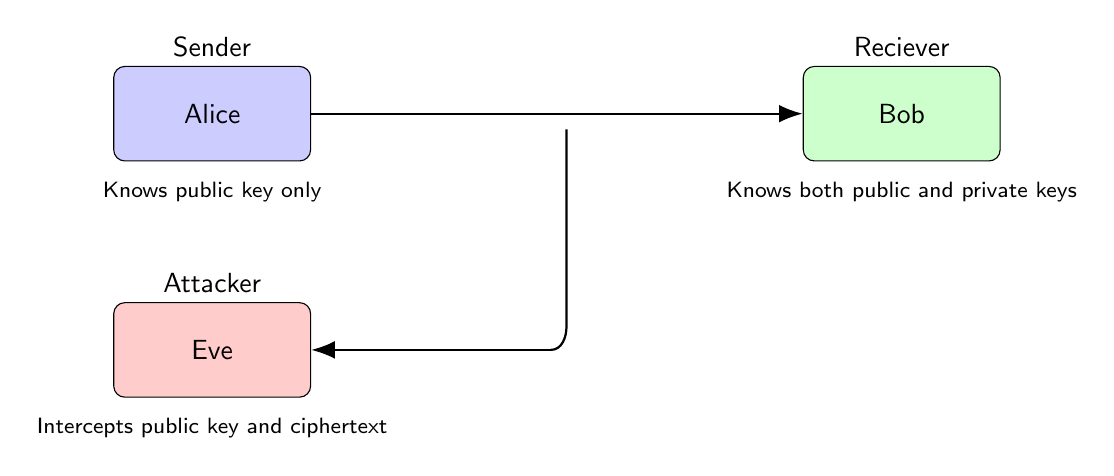
\begin{tikzpicture}[node distance=1.7cm and 1.5cm, font=\sffamily,
    every node/.style={align=center},
    box/.style={rectangle, draw, rounded corners, minimum width=2.5cm, minimum height=1.2cm},
    box1/.style={box, fill=blue!20},
    box2/.style={box, fill=red!20},
    box3/.style={box, fill=green!20},
    arrow/.style={-{Latex[length=3mm]}, thick},
]



\node[box1,label=above:{Sender}] (alice) at (-3, 0) {Alice};
\node[below=4pt of alice] {\footnotesize Knows public key only};

\node[box2,label = above:{Attacker}] (eve) at (-3, -3) {Eve};
\node[below=4pt of eve] {\footnotesize Intercepts public key and ciphertext};

\node[box3, right=of alice, label = above:{Reciever}] (bob) at (3, 0) {Bob};

\node[below=4pt of bob] {\footnotesize Knows both public and private keys};


\draw[arrow] (alice) -- (bob);

%\draw[arrow] (1.5,0) to[bend left=45] (eve.east);

\draw[arrow, -]
  (1.5,-0.2) -- ++(0,-2.5) 
  to[out=270,in=0,looseness=1] (1.3,-3);
 
 \draw[arrow]
  (1.3,-3) -- (eve.east);

\end{tikzpicture}

\textbf{Figure 4.} Visualization of the LLL-based attack on RSA , where Eve intercepts the message sent from Alice to Bob.
\end{center}


Alice wants to send Bob a message of the form

\begin{center}
\textit{The answer is **}
\end{center}

or

\begin{center}
\textit{The password for your new account is ********.}
\end{center}

In these cases, the message is of the form
\[
m = B + x, \quad \text{where } B \text{ is fixed and } |x| \leq Y
\]
for some integer $Y$. We'll present an attack that works when the encryption exponent is small.


\medskip

Suppose Bob has public RSA key $(n,e) = (n,3)$. Then the ciphertext is
\[
c \equiv (B + x)^3 \pmod{n}.
\]

We assume that Eve knows $B$, $Y$, and $n$, so she only needs to find $x$. She forms the polynomial
\[
f(T) = (B + T)^3 - c = T^3 + 3BT^2 + 3B^2T + B^3 - c
\equiv T^3 + a_2 T^2 + a_1 T + a_0 \pmod{n}.
\]

Eve is looking for $|x| \leq Y$ such that $f(x) \equiv 0 \pmod{n}$. In other words, she is looking for a small solution to a polynomial congruence $f(T) \equiv 0 \pmod{n}$.

Eve applies the \textit{LLL} algorithm to the lattice generated by the vectors
\[
\begin{aligned}
v_1 &= (n, 0, 0, 0), \\
v_2 &= (0, Yn, 0, 0), \\
v_3 &= (0, 0, Y^2n, 0), \\
v_4 &= (a_0, a_1Y, a_2Y^2, Y^3).
\end{aligned}
\]

This yields a new basis $b_1, \dots, b_4$, but we need only $b_1$. The theorem in Subsection~2.3 tells us that
\[
\|b_1\| \leq 2^{3/4} \det(v_1,\dots,v_4)^{1/4}
= 2^{3/4}(n^3Y^6)^{1/4} = 2^{3/4}n^{3/4}Y^{3/2}. \tag{17.3}
\]

We can write

\[
b_1 = c_1v_1 + \cdots + c_4v_4 = (e_0, Y e_1, Y^2 e_2, Y^3 e_3)
\]
with integers $c_i$ and with
\[
\begin{aligned}
e_0 &= c_1 n + c_4 a_0, \\
e_1 &= c_2 n + c_4 a_1, \\
e_2 &= c_3 n + c_4 a_2, \\
e_3 &= c_4.
\end{aligned}
\]

We observe that the coefficients \( e_i \) of the polynomial \( g(T) \) satisfy
\[
e_i \equiv c_4 a_i \pmod{n}, \quad \text{for } i = 0, 1, 2.
\]

Now, define the polynomial
\[
g(T) = e_3 T^3 + e_2 T^2 + e_1 T + e_0.
\]

Since \( x \) is a root of \( f(T) \) modulo \( n \), and \( g(T) \equiv c_4 f(T) \mod n \), we have:
\[
g(x) \equiv 0 \pmod{n}.
\]

Assume that
\[
Y < 2^{-7/6} n^{1/6}. \tag{17.4}
\]

We now estimate the size of \( g(x) \):
\[
\begin{aligned}
|g(x)| &\leq |e_0| + |e_1 x| + |e_2 x^2| + |e_3 x^3| \\
       &\leq |e_0| + |e_1|Y + |e_2|Y^2 + |e_3|Y^3 \\
       &= \langle (1, 1, 1, 1), (|e_0|, |e_1 Y|, |e_2 Y^2|, |e_3 Y^3|) \rangle \\
       &\leq \|(1,1,1,1)\| \cdot \|(|e_0|, |e_1 Y|, |e_2 Y^2|, |e_3 Y^3|)\| \\
       &= 2 \|b_1\|,
\end{aligned}
\]
where we used the Cauchy–Schwarz inequality in the last step.

Using the bound from inequality (17.3) and our assumption (17.4), we get
\[
\|b_1\| \leq 2^{3/4} n^{3/4} Y^{3/2} < 2^{3/4} n^{3/4} \left(2^{-7/6} n^{1/6}\right)^{3/2} = \frac{n}{2}.
\]

Therefore,
\[
|g(x)| < n.
\]

Given method transforms the modular equation \( f(T) \equiv 0 \pmod{n} \) into an exact polynomial equation \( g(T) = 0 \), which can be solved numerically. At most three candidates for \( x \) are tested to recover the plaintext. More generally, small roots of modular equations can be found using LLL on a lattice of dimension \( d+1 \). Coppersmith's method extends this to polynomials of degree \( d \), allowing recovery of \( x \) when \( |x| \leq n^{1/d} \), in polynomial time.


 This attack method is based on the description from the book \textit{Introduction to Cryptography with Coding Theory} by Trappe and Washington (2nd Edition, Pearson, 2006). An example implementation of this attack has been developed and published by the author on GitHub: \href{https://github.com/SanyaKor/Cryptanalysis/blob/main/notebooks/lll\_attack.ipynb}{github.com/SanyaKor/Cryptanalysis/blob/main/notebooks/lll\_attack.ipynb}.
\newpage

\subsection{NTRU}

Lattice-based cryptography becomes especially powerful in high-dimensional settings. While traditional reduction techniques like the \textsc{LLL} algorithm lose their effectiveness as the dimension \( n \) increases (typically beyond \( n \geq 100 \)), this limitation opens the door for new constructions that rely on the hardness of certain lattice problems.

One of the most prominent lattice-based cryptosystems is \textsc{NTRU}, a public-key encryption scheme known for its efficiency and resistance to quantum attacks. Although its original formulation did not explicitly reference lattices, it can be naturally interpreted through a lattice framework—a perspective we will explore in this chapter.

\bigskip

\subsection*{Preliminaries for NTRU}
Before presenting the structure of the NTRU cryptosystem, we introduce a few algebraic preliminaries.

We work with polynomials of degree less than \( N \), with coefficients in the ring \( \mathbb{Z}_q \). Let

\[
f(x) = \sum_{i=0}^{N-1} a_i x^i, \qquad g(x) = \sum_{i=0}^{N-1} b_i x^i
\]

be two such polynomials. Their ordinary (non-reduced) product over \( \mathbb{Z} \) is given by:

\[
(f * g)(x) = \sum_{k=0}^{2N-2} \left( \sum_{i=0}^k a_i b_{k-i} \right) x^k.
\]

However, NTRU operates in the quotient ring \( \mathbb{Z}_q[x]/(x^N - 1) \), where coefficients are reduced modulo \( q \), and the exponents wrap around modulo \( N \). In this ring, polynomial multiplication becomes

\[
(f \ast g)(x) = \sum_{i=0}^{N-1} c_i x^i, \qquad \text{where } c_i = \sum_{\substack{j + k \equiv i \!\!\!\! \pmod{N}}} a_j b_k \pmod{q}.
\]

This cyclic convolution is fundamental to the design and efficiency of the NTRU cryptosystem.

\medskip
\begin{example}
Let \( N = 3 \), and consider the polynomials
\[
f(x) = x^2 + 7x + 9, \qquad g(x) = 3x^2 + 2x + 5.
\]
We compute their cyclic convolution product \( f \ast g \) in \( \mathbb{Z}[x]/(x^3 - 1) \). The coefficient \( c_1 \) of \( x \) is

\[
c_1 = a_0 b_1 + a_1 b_0 + a_2 b_2 = 9 \cdot 2 + 7 \cdot 5 + 1 \cdot 3 = 56,
\]

and the full product is

\[
f \ast g = 46x^2 + 56x + 68.
\]
\end{example}

\smallskip
\noindent
An implementation of this polynomial multiplication is available on GitHub:  
\href{https://github.com/SanyaKor/Cryptanalysis/blob/main/lattice\_methods/ntru.py}{\texttt{github.com/SanyaKor/Cryptanalysis/blob/main/lattice\_methods/ntru.py}}

\smallskip
\noindent\textbf{Addition.}
Given two polynomials
\[
f(x) = \sum_{i=0}^{N-1} a_i x^i, \quad g(x) = \sum_{i=0}^{N-1} b_i x^i,
\]
their sum in \( \mathbb{Z}_q[x]/(x^N - 1) \) is defined coefficient-wise:
\[
(f + g)(x) = \sum_{i=0}^{N-1} (a_i + b_i \bmod q)\, x^i.
\]
This operation is straightforward and preserves the ring structure.


\medskip
\noindent
NTRU works with a specific subset of polynomials that have small integer coefficients. To formalize this, we define a family of sets:

\[
\mathcal{L}(j, k) = 
\left\{
  \begin{array}{l}
    \text{the set of polynomials of degree } < N \text{ with} \\
    j \text{ coefficients equal to } +1,\ k \text{ coefficients equal to } -1, \\
    \text{and all other coefficients equal to } 0.
  \end{array}
\right.
\]
The remaining coefficients are set to zero.

\medskip

\noindent
We are now ready to describe the NTRU cryptosystem. Suppose Alice wishes to send a message to Bob. To begin, Bob must generate and publish a public key. He selects three integers \( N, p, q \), subject to the constraints:
\[
\gcd(p, q) = 1, \quad \text{and} \quad p \ll q.
\]
Recommended parameters for moderate security include:
\[
(N, p, q) = (107, 3, 64),
\]
and for higher security:
\[
(N, p, q) = (503, 3, 256).
\]

\begin{table}[h!]
\centering
\begin{tabular}{|c|c|c|c|c|c|}
\hline
\textbf{Case} & \textbf{Level} & \boldmath$N$ & \boldmath$p$ & \boldmath$q$ & \textbf{Time (seconds)} \\
\hline
A & Moderate & 107 & 3 & 64 & $780,\!230$ (9 days) \\
\hline
B & High & 167 & 3 & 128 & $1.198 \cdot 10^{10}$ (380 years) \\
\hline
C & Highest & 503 & 3 & 256 & $1.969 \cdot 10^{35}$ ($6.2 \cdot 10^{27}$ years) \\
\hline
\end{tabular}
\end{table}

NTRU Parameter Sets and Estimated Attack Times. Based on data from \url{https://www.ntru.org/}. Tests were performed on a 200 MHz Pentium Pro processor.

\newpage

To initiate the cryptosystem, Bob begins by selecting two small polynomials \( f \) and \( g \), typically with coefficients in \(\{-1, 0, 1\}\). These polynomials are chosen such that \( f \) is invertible modulo both \( p \) and \( q \). This means there exist polynomials \( F_p \) and \( F_q \), each of degree less than \( N \), such that

\[
F_p * f \equiv 1 \pmod{p}, \qquad F_q * f \equiv 1 \pmod{q}.
\]

Using these, Bob computes the public key polynomial

\[
h \equiv F_q * g \pmod{q},
\]

and publishes the tuple \( (N, p, q, h) \) as his public key.

\medskip

The private key is the polynomial \( f \), which should be kept secret. Although \( F_p \) can be efficiently recomputed from \( f \), it is recommended to store it for faster decryption. As for \( g \), note that since \( g \equiv f * h \pmod{q} \), all required information is contained in \( f \) and \( h \), so storing \( g \) is unnecessary.


\subsection*{Encryption and Decryption in NTRU}

Once the keys are established, Alice can encrypt a message for Bob. She encodes her message as a polynomial \( m \) of degree less than \( N \), with coefficients from \( \{ -1, 0, 1 \} \), assuming \( p = 3 \). Then she chooses a small random polynomial \( \phi \) (its precise constraints will be detailed later) and computes the ciphertext as

\[
c \equiv p\phi * h + m \pmod{q}.
\]

This ciphertext \( c \) is sent to Bob.

\medskip

To decrypt the message, Bob first computes

\[
a \equiv f * c \pmod{q}.
\]

If all coefficients of \( a \) have absolute value less than \( q/2 \), he can recover the original message by reducing modulo \( p \):

\[
m \equiv F_p * a \pmod{p}.
\]


Although decryption is not always guaranteed to succeed, appropriate parameter choices yield very low failure probabilities (e.g., less than \( 5 \times 10^{-5} \)).

Here’s a sketch of why decryption usually works:

\[
a \equiv f * c \equiv f * (p\phi * h + m) \equiv f * p\phi * F_q * g + f * m \equiv p\phi * g + f * m \pmod{q}.
\]

Given that \( \phi, g, f, m \) all have small coefficients and \( p \ll q \), it is likely that the result does not wrap modulo \( q \), so we can treat the expression as:

\[
a = p\phi * g + f * m.
\]

Applying \( F_p \), we have:

\[
F_p * a = pF_p * \phi * g + F_p * f * m \equiv 0 + 1 * m \equiv m \pmod{p},
\]

which successfully recovers the message \( m \).




\medskip

A complete implementation of the NTRU cryptosystem, including key generation, encryption, and decryption, is available on GitHub:  
\href{https://github.com/SanyaKor/Cryptanalysis/blob/main/lattice\_methods/ntru.py}{\texttt{github.com/SanyaKor/Cryptanalysis/blob/main/lattice\_methods/ntru.py}}

\smallskip

An example demonstrating how to use the NTRU scheme in practice can be found at:  
\href{https://github.com/SanyaKor/Cryptanalysis/blob/main/notebooks/usage_examples.ipynb}{\texttt{notebooks/usage\_examples.ipynb}}

\medskip

\subsection*{Advantages and Disadvantages of NTRU}

\textbf{Advantages:}
\begin{itemize}
  \item \textit{Efficiency:} NTRU offers fast key generation, encryption, and decryption compared to many other public-key schemes.
  \item \textit{Small Key Sizes:} Public and private keys are relatively small, making NTRU attractive for constrained environments.
  \item \textit{Post-Quantum Security:} NTRU is believed to be resistant to attacks by quantum computers, unlike RSA or ECC.
\end{itemize}

\textbf{Disadvantages:}
\begin{itemize}
  \item \textit{Decryption Failures:} With improper parameters, decryption can fail. Careful tuning is required.
  \item \textit{Parameter Sensitivity:} Security and correctness heavily depend on choosing parameters properly.
  \item \textit{Lattice Attacks:} Though generally secure, NTRU remains susceptible to advanced lattice-based attacks if parameters are too weak.
\end{itemize}

\newpage

\subsection{Attack on NTRU}

Let \( h = h_{N-1}X^{N-1} + \cdots + h_0 \). Form the \( N \times N \) matrix
\[
H = 
\begin{pmatrix}
h_0     & h_1     & \cdots & h_{N-1} \\
h_{N-1} & h_0     & \cdots & h_{N-2} \\
\vdots  & \vdots  & \ddots & \vdots  \\
h_1     & h_2     & \cdots & h_0
\end{pmatrix}.
\]

If we represent the polynomials \( f = f_{N-1}X^{N-1} + \cdots + f_0 \) and \( g = g_{N-1}X^{N-1} + \cdots + g_0 \) by their corresponding row vectors:
\[
\vec{f} = (f_0, \dots, f_{N-1}), \quad \vec{g} = (g_0, \dots, g_{N-1}),
\]
then multiplication in \( \mathbb{Z}_q[x]/(x^N - 1) \) can be viewed as matrix-vector multiplication \( H \cdot \vec{f} \).

\vspace{0.5em}

Here, \( H \) is a circulant matrix generated from the coefficients of \( h \). This form is particularly useful because circulant matrices encode convolution-like operations. When working modulo \( X^N - 1 \), the multiplication of polynomials behaves like cyclic convolution. Representing this operation via matrix multiplication simplifies both notation and implementation, especially in lattice-based cryptographic schemes like NTRU.


We observe that
\[
\vec{f} H \equiv \vec{g} \pmod{q}.
\]

To express this relationship as a lattice problem, define the identity matrix \( I \) and the scaled identity matrix \( qI \) as:
\[
I =
\begin{pmatrix}
1 & 0 & \cdots & 0 \\
0 & 1 & \cdots & 0 \\
\vdots & \vdots & \ddots & \vdots \\
0 & 0 & \cdots & 1
\end{pmatrix}, \qquad
qI =
\begin{pmatrix}
q & 0 & \cdots & 0 \\
0 & q & \cdots & 0 \\
\vdots & \vdots & \ddots & \vdots \\
0 & 0 & \cdots & q
\end{pmatrix}.
\]

Now form the \( 2N \times 2N \) matrix \( M \) by:
\[
M = 
\begin{pmatrix}
I & H \\
0 & qI
\end{pmatrix}.
\]

Let \( y \) be an unknown polynomial of degree less than \( N \), with coefficient vector \( \vec{y} \). Then we can express the relation
\[
g = f * h + qy
\]
as
\[
(\vec{f}, \vec{y}) M = (\vec{f}, \vec{g}).
\]

This means the vector \( (\vec{f}, \vec{g}) \) belongs to the lattice \( L \) generated by the rows of \( M \). Because \( f \) and \( g \) have small coefficients, the corresponding vector is short. An attacker can apply lattice reduction techniques (like the LLL algorithm) to search for short vectors in \( L \), and potentially recover \( f \) and \( g \), thus compromising the cryptosystem.
%%%%%%%%%%%%%%%%%%%%%%%%%%%%%%%%%%%%%%%%%%%%%%%

%%%%%%%%%%%%%%%%%%%%%%%%%%%%%%%%%%%%%%%%%%%%%%%
\newpage
\section{Code}
This section provides an overview of the source code modules responsible for implementing the core functionality of the project.It includes core algorithms for lattice manipulation, polynomial arithmetic, cryptographic operations,  
and supporting utilities such as testing and verification routines.

Each file is presented with its key functions, their parameters, return types, and the full implementation  
as extracted directly from the Python source. The structure is modular, with each component focusing on  
a specific aspect of the overall system.

\vspace{1em}
\noindent
\textbf{Note:} This documentation includes only the main functions.  
Some helper or internal code is not shown here.  
To explore the full project, including all source files and examples, visit the GitHub repository:  
\texttt{https://github.com/SanyaKor/Cryptanalysis}

\subsection{Lattice Methods}
This section contains core functions for lattice-based computations, including basis reduction,  
coefficient normalization, and algebraic operations over polynomial rings.  
These methods form the foundation of the cryptographic and algorithmic procedures implemented in this project.

All functions are implemented in Python and designed to be modular and reusable across different schemes.
\subsubsection{basis\_reduction\_2d}

\section*{Function: \texttt{reduce\_2d\_basis}}

\textbf{Description:}

Performs Gauss-style reduction of a 2D lattice basis.

This function reduces a two-dimensional lattice basis using a simplified form
of Gauss' lattice basis reduction algorithm. The process iteratively subtracts
integer multiples of vectors to produce a shorter, more orthogonal basis.
\vspace{1em}
\noindent
\textbf{Parameters:}

\vspace{0.5em}
\begin{tabular}{p{3cm} p{11cm}}
\texttt{basis1} & \texttt{numpy.ndarray} — First basis vector. \\
\texttt{basis2} & \texttt{numpy.ndarray} — Second basis vector. \\
\texttt{verbose} & \texttt{bool} — If True, returns a log of each reduction step. \\
\end{tabular}

\vspace{1em}
\noindent
\textbf{Returns:}

\vspace{0.5em}
\begin{tabular}{p{3cm} p{11cm}}
\texttt{return} & \texttt{list} — If \texttt{verbose} is False, returns \texttt{[b1, b2]} (the reduced basis).\\
                & If \texttt{verbose} is True, returns a list of dictionaries with step-by-step logs:\\
                & \quad • \texttt{step} — step index or ``$\rightarrow$ shortest''\\
                & \quad • \texttt{b1}, \texttt{b2} — current reduced basis vectors (NumPy arrays).\\
\end{tabular}

\vspace{1em}
\noindent
\textbf{Note:}  
The algorithm stops when the projection coefficient \texttt{t} becomes zero.  
This is a simplified form of Gauss’ lattice basis reduction in 2D.

\textbf{Source Code:}

\begin{lstlisting}[language=Python]
def reduce_2d_basis(basis1, basis2, verbose=False):
    data = []

    steps = 0

    #TODO linear ind check
    # if np.linalg.matrix_rank(np.column_stack((basis1, basis2))) < 2:
    #     raise ValueError("Input vectors are linearly dependent.")

    while True:

        if np.linalg.norm(basis2) < np.linalg.norm(basis1):
            basis1, basis2 = basis2, basis1
            continue


        t = round(np.dot(basis1, basis2) / np.dot(basis1, basis1))

        data.append({
            'step': steps,
            'b1': basis1.copy(),
            'b2': basis2.copy(),
        })

        steps += 1


        if t == 0:
            break

        basis2 = basis2 - t * basis1

    shortest = basis1 if np.linalg.norm(basis1) <= np.linalg.norm(basis2) else basis2

    ###TODO reducing the basis not includes short vector, might have to remove
    data.append({
        'step': ' shortest',
        'b1': shortest if np.array_equal(shortest, basis1) else '',
        'b2': shortest if np.array_equal(shortest, basis2) else ''
    })

    return data if verbose else [basis1, basis2]
\end{lstlisting}



%%%%%%%%%%%%%%%%%%%%%%%%%%%%%%%%%%%%%%%%%%%%%%%

%%%%%%%%%%%%%%%%%%%%%%%%%%%%%%%%%%%%%%%%%%%%%%%


\subsubsection{lll}

\section*{Function: \texttt{lll\_reduce}}

\textbf{Description:}

Performs LLL (Lenstra–Lenstra–Lovász) lattice basis reduction.

This function applies the classical LLL algorithm to reduce a given lattice basis
to a shorter and nearly orthogonal form.

\vspace{1em}
\noindent
\textbf{Parameters:}

\vspace{0.5em}
\begin{tabular}{p{3cm} p{11cm}}
\texttt{basis} & list[\texttt{numpy.ndarray}] — A list of NumPy vectors representing the lattice basis. \\
\texttt{delta} & float — Lovász parameter, typically in the range (0.5, 1). Default is 0.75. \\
\texttt{verbose} & bool — If True, enables step-by-step debug output (currently unused). \\
\end{tabular}

\vspace{1em}
\noindent
\textbf{Returns:}

\vspace{0.5em}
\begin{tabular}{p{3cm} p{11cm}}
\texttt{return} & list[\texttt{numpy.ndarray}] — A list of NumPy vectors representing the LLL-reduced lattice basis. \\
\end{tabular}

\vspace{1em}
\noindent
\textbf{Note:}  
This function assumes all basis vectors are linearly independent.

\vspace{1em}
\noindent
\textbf{Warning:}  
No validation is performed on the input; ensure basis vectors are valid.

\vspace{1em}
\noindent
\textbf{See also:}  
\texttt{lattice\_methods.utils.gram\_schmidt} for orthogonalization.

\begin{lstlisting}[language=Python]
def lll_reduce(basis, delta=0.75, verbose=False):

    ##TODO verbose ..

    basis = [b.copy() for b in basis]
    n = len(basis)
    k = 1


    while k < n:

        ortho, mu = gram_schmidt(basis)

        for j in range(k - 1, -1, -1):  # j < k

            if abs(mu[k, j]) > 0.5:
                r = round(mu[k, j])
                basis[k] -= r * basis[j]
                ortho, mu = gram_schmidt(basis)

        norm_sq_prev = np.dot(ortho[k - 1], ortho[k - 1])
        norm_sq_curr = np.dot(ortho[k], ortho[k])

        lhs = delta * norm_sq_prev
        rhs = norm_sq_curr + mu[k, k - 1]**2 * norm_sq_prev

        if lhs > rhs:
            basis[k], basis[k - 1] = basis[k - 1], basis[k].copy()

            k = max(k - 1, 1)
        else:
            k += 1

    return basis
\end{lstlisting}







%%%%%%%%%%%%%%%%%%%%%%%%%%%%%%%%%%%%%%%%%%%%%%%

%%%%%%%%%%%%%%%%%%%%%%%%%%%%%%%%%%%%%%%%%%%%%%%




\subsubsection{ntru}

\section*{Function: \texttt{poly\_inv\_mod\_ring}}

\textbf{Description:}

Computes the inverse of a polynomial modulo (pow(x,N) - 1) and q.

This function attempts to find the inverse of a given polynomial `polynomial$\_$f` in the ring
of polynomials modulo (pow(x,N) - 1) with coefficients reduced modulo `q`. It works both when `q`
is prime and composite by setting the appropriate polynomial domain.

\vspace{1em}

\textbf{Parameters:}

\vspace{1em}
\noindent
\begin{tabular}{p{3cm} p{11cm}}
\texttt{polynomial\_f} & sympy.Poly — The polynomial to invert (as a SymPy Poly object). \\
\texttt{N} & int — The degree defining the modulus polynomial pow(x,N) - 1. \\
\texttt{q} & int — The modulus for coefficient arithmetic. \\
\end{tabular}

\vspace{1em}
\noindent
\textbf{Returns:}

\begin{tabular}{p{3cm} p{11cm}}
\texttt{return} & list[int] or None — List of coefficients of the inverse polynomial if it exists; otherwise, None. \\
\end{tabular}

\vspace{1em}
\textbf{Source Code:}

\begin{lstlisting}
def poly_inv_mod_ring(polynomial_f, N, q):

    #f = Poly(f_coeffs, x, domain=GF(q))
    if(isprime(q)):
        mod_poly = Poly(x**N - 1, x, domain=GF(q))
    else:
        mod_poly = Poly(x ** N - 1, x, domain=ZZ).trunc(q)

    polynomial_f = polynomial_f.set_domain(mod_poly.domain)

    if gcd(polynomial_f, mod_poly).degree() != 0:
        return None

    try:
        inv = invert(polynomial_f, mod_poly)
        return inv.all_coeffs()
    except Exception:
        return None
\end{lstlisting}

\section*{Function: \texttt{poly\_mult\_mod\_ring}}

\textbf{Description:}

Performs multiplication of two polynomials modulo (pow(x,N) - 1) and coefficient modulus q.

This function computes the product of two polynomials represented by coefficient lists `p1` and `p2`.
The multiplication is done modulo the polynomial (pow(x,N) - 1), which means the coefficients
are reduced with wrap-around at degree N, and all coefficients are taken modulo `q`.

\vspace{1em}

\textbf{Parameters:}

\vspace{1em}
\noindent
\begin{tabular}{p{3cm} p{11cm}}
\texttt{p1} & list[int] — Coefficients of the first polynomial (highest degree first). \\
\texttt{p2} & list[int] — Coefficients of the second polynomial (highest degree first). \\
\texttt{N} & int — Degree of the modulus polynomial (pow(x,N) - 1). \\
\texttt{q} & int — Modulus for coefficient arithmetic. \\
\end{tabular}

\vspace{1em}
\noindent
\textbf{Returns:}

\begin{tabular}{p{3cm} p{11cm}}
\texttt{return} & list[int] — Coefficients of the resulting polynomial after modular multiplication, \\
\end{tabular}

\vspace{1em}
\textbf{Source Code:}

\begin{lstlisting}[language=Python]
def poly_mult_mod_ring(p1, p2, N, q):
    p1 = p1[::-1]
    p2 = p2[::-1]

    length = len(p1) + len(p2) - 1
    result = [0] * length
    for i in range(len(p1)):
        for j in range(len(p2)):
            idx = (i + j)
            result[idx] += p1[i] * p2[j]

    for i in range(len(result)):
        if(i > N-1):
            difference = i % N
            result[difference] += result[i]
            result[i] = 0

    for i in range(len(result)-1, -1, -1):
        if(result[i]!=0 or len(result) <= N):
            break

        result.pop(i)

    return [c % q for c in result[::-1]]
\end{lstlisting}

\section*{Function: \texttt{ntru\_generate\_keys}}

\textbf{Description:}

Generates public and private keys for the NTRU cryptosystem.

This function computes the NTRU key pair based on parameters N, p, q and the
private polynomials `polynomial$\_$f` and `polynomial$\_$g`. It returns the public key
and the inverse of `polynomial$\_$f` modulo q, which serves as part of the private key.

\vspace{1em}
\textbf{Parameters:}

\vspace{1em}
\noindent
\begin{tabular}{p{3cm} p{11cm}}
\texttt{N} & int — Degree of the polynomials and ring dimension. \\
\texttt{p} & int — Small modulus parameter for message space. \\
\texttt{q} & int — Large modulus parameter for polynomial arithmetic. \\
\texttt{polynomial\_g} & sympy.Poly — Polynomial used in key generation (SymPy Poly). \\
\texttt{polynomial\_f} & sympy.Poly — Private polynomial used for key generation (SymPy Poly). \\
\end{tabular}

\vspace{1em}
\noindent
\textbf{Returns:}

\begin{tabular}{p{3cm} p{11cm}}
\texttt{return} & tuple[list, list] — Tuple `(pub$\_$key, prv$\_$key)` where \\
\end{tabular}

\vspace{1em}
\textbf{Source Code:}

\begin{lstlisting}[language=Python]
def ntru_generate_keys(N : int, p: int, q : int, polynomial_g : Poly, polynomial_f : Poly):

    if(gcd(p, q) != 1 or p >= q):
        print("ERROR SMTH WRONG WITH p, q ")
        return

    if(isprime(q)):
        poly_f_over_q = Poly(polynomial_f, x, domain=GF(q))
    else:
        poly_f_over_q = Poly(polynomial_f, x, domain=ZZ).trunc(q)

    poly_f_over_p = Poly(polynomial_f, x, domain=GF(p))

    Fp = poly_inv_mod_ring(poly_f_over_p, N, p)
    Fq = poly_inv_mod_ring(poly_f_over_q, N, q)

    if Fp is None or Fq is None:
        print("ERROR SMTH WRONG WITH POLYNOMIALS Fq Fp")
        return

    Fqp = [p * x for x in Fq]
    h = poly_mult_mod_ring(Fqp, polynomial_g.all_coeffs(), N, q)

    pub_key = [N, p, q, h]
    prv_key = [polynomial_f, Fp]

    return pub_key, prv_key
\end{lstlisting}

\section*{Function: \texttt{ntru\_encryption}}

\textbf{Description:}

Encrypts a message polynomial using the NTRU public key.

This function performs NTRU encryption by computing the ciphertext polynomial as
the sum of the product of the random polynomial `polynomial$\_$phi` with the public key polynomial `h`,
plus the message polynomial `polynomial$\_$m`, all modulo `q`.

\vspace{1em}
\textbf{Parameters:}

\vspace{1em}
\noindent
\begin{tabular}{p{3cm} p{11cm}}
\texttt{pubkey} & list — Public key represented as a list `[N, p, q, h]`. \\
\texttt{polynomial\_phi} & sympy.Poly — Random polynomial used for encryption (SymPy Poly). \\
\texttt{polynomial\_m} & sympy.Poly — Message polynomial to encrypt (SymPy Poly). \\
\end{tabular}

\vspace{1em}
\noindent
\textbf{Returns:}

\begin{tabular}{p{3cm} p{11cm}}
\texttt{return} & list[int] — Ciphertext polynomial coefficients modulo q. \\
\end{tabular}

\vspace{1em}
\textbf{Source Code:}

\begin{lstlisting}[language=Python]
def ntru_encryption(pubkey, polynomial_phi: Poly, polynomial_m: Poly):
    N, p, q, h = pubkey

    phi_coeffs = polynomial_phi.all_coeffs()
    m_coeffs = polynomial_m.all_coeffs()

    c = poly_mult_mod_ring(phi_coeffs, h, N, q)
    ciphertext = poly_add_mod_ring(c, m_coeffs, q)

    return ciphertext
\end{lstlisting}

\section*{Function: \texttt{ntru\_decryption}}

\textbf{Description:}

Decrypts a ciphertext polynomial using the NTRU private key.

This function performs NTRU decryption by multiplying the ciphertext with the private
polynomial `polynomial$\_$f` modulo (pow(x,N) - 1, q), centering the coefficients if needed,
and then multiplying by the inverse of `polynomial$\_$f` modulo p to recover the original message polynomial.

\vspace{1em}
\textbf{Parameters:}

\vspace{1em}
\noindent
\begin{tabular}{p{3cm} p{11cm}}
\texttt{pubkey} & list — Public key represented as a list `[N, p, q, h]`. \\
\texttt{prvkey} & list — Private key represented as a list `[polynomial$\_$f, Fp]`, \\
\texttt{ciphertext} & list[int] — Ciphertext polynomial coefficients. \\
\end{tabular}

\vspace{1em}
\noindent
\textbf{Returns:}

\begin{tabular}{p{3cm} p{11cm}}
\texttt{return} & sympy.Poly — Decrypted message polynomial over GF(p). \\
\end{tabular}

\vspace{1em}
\textbf{Source Code:}

\begin{lstlisting}[language=Python]
def ntru_decryption(pubkey, prvkey, ciphertext):
    [polynomial_f, Fp] = prvkey
    N, p, q, h = pubkey

    f_coeffs = polynomial_f.all_coeffs()
    a = poly_mult_mod_ring(f_coeffs, ciphertext, N, q)

    cond = check_coeff_range(a, (-q/2, q/2))
    if not cond:
        a = center_poly_coeffs(a, q)

    Fpa = poly_mult_mod_ring(Fp, a, N, p)
    #print(Poly(Fpa, x, domain=GF(p)))

    return Poly(Fpa, x, domain=GF(p))
\end{lstlisting}



%%%%%%%%%%%%%%%%%%%%%%%%%%%%%%%%%%%%%%%%%%%%%%%

%%%%%%%%%%%%%%%%%%%%%%%%%%%%%%%%%%%%%%%%%%%%%%%


\subsection{Tests}

This section provides the core test functions used to verify the behavior of the implemented lattice algorithms.  
Each function performs automated checks on correctness and expected improvements after reduction.

For complete source code and additional test cases, see the full repository on GitHub. 
\noindent
\href{https://github.com/SanyaKor/Cryptanalysis/tree/main/tests}{\texttt{Cryptanalysis/tests} on GitHub}
\\



\subsubsection{tests\_br2d}

\section*{Function: \texttt{tests\_br2d}}

\textbf{Description:}

Performs batch testing of 2D lattice basis reduction.

This function takes a list of 2D lattice bases, applies the `reduce$\_$2d$\_$basis` algorithm to each pair,
and verifies two conditions for each reduction:
  1. The reduced basis is equivalent to the original basis.
  2. The shorter vector in the reduced basis is no longer than in the original.

A test is marked as passed only if both conditions hold.

\vspace{1em}
\textbf{Parameters:}

\vspace{1em}
\noindent
\begin{tabular}{p{3cm} p{11cm}}
\texttt{basis\_list} & list[tuple[np.ndarray, np.ndarray]] — List of 2D lattice bases. Each element is a pair of vectors (b1, b2), where b1 and b2 are NumPy arrays. \\
\texttt{verbose} & bool — Whether to print detailed output for each test. \\
\end{tabular}

\vspace{1em}
\noindent
\textbf{Returns:}

\begin{tabular}{p{3cm} p{11cm}}
\texttt{return} & list[dict[str, Any]] — List of test results. Each result is a dict with reduced vectors and a pass/fail flag. \\
\end{tabular}

\vspace{1em}
\textbf{Source Code:}

\begin{lstlisting}[language=Python]
def tests_br2d(basis_list, verbose=False):
    tests_amount = len(basis_list)
    tests_passed = 0

    results = []

    for i, (b1, b2) in enumerate(basis_list):

        b1_reduced, b2_reduced = reduce_2d_basis(b1, b2)

        same = are_bases_equivalent([b1, b2], [b1_reduced, b2_reduced])

        original_len = min(np.linalg.norm(b1), np.linalg.norm(b2))
        reduced_len = min(np.linalg.norm(b1_reduced), np.linalg.norm(b2_reduced))
        improved = reduced_len <= original_len

        if same and improved:
            tests_passed += 1
            if verbose:
                print(f" Test {i + 1}: PASSED")
                print(f"Initial basis: b1 = {b1}, b2 = {b2}")
                print(f"Reduced basis: b1 = {b1_reduced}, b2 = {b2_reduced}")

            results.append({
                "b1": b1_reduced,
                "b2": b2_reduced,
                "result": 1
            })

        else:

            if verbose:
                print(f" Test {i + 1} FAILED: ")
                print(f"b1 = {b1}, b2 = {b2}")

            results.append({
                    "b1": b1_reduced,
                    "b2": b2_reduced,
                    "result": 0
            })
    if verbose:
        print(f"\n {tests_amount}/{tests_passed} tests passed.")

    return results
\end{lstlisting}




%%%%%%%%%%%%%%%%%%%%%%%%%%%%%%%%%%%%%%%%%%%%%%%

%%%%%%%%%%%%%%%%%%%%%%%%%%%%%%%%%%%%%%%%%%%%%%%


\subsubsection{tests\_lll}

\section*{Function: \texttt{tests\_brlll}}

\textbf{Description:}

Performs batch testing of LLL lattice basis reduction.

This function takes a list of lattice bases, applies the LLL reduction
algorithm to each, and verifies two key properties:
  1. The reduced basis is equivalent to the original one.
  2. The shortest vector in the reduced basis is no longer than in the original.

Each test is counted as passed if both properties hold.

\vspace{1em}
\newpage
\textbf{Parameters:}

\vspace{1em}
\noindent
\begin{tabular}{p{3cm} p{11cm}}
\texttt{basis\_list} & list[list[np.ndarray]] — List of lattice bases to test. Each basis is a list of NumPy arrays. \\
\texttt{verbose} & bool — Whether to print step-by-step output for each test. \\
\end{tabular}

\vspace{1em}
\noindent
\textbf{Returns:}

\begin{tabular}{p{3cm} p{11cm}}
\texttt{return} & list[dict[str, Any]] — List of results per test. Each result is a dict with the reduced basis and pass/fail flag. \\
\end{tabular}

\textbf{Source Code:}

\begin{lstlisting}[language=Python]
def tests_brlll(basis_list, verbose=False):
    tests_amount = len(basis_list)
    tests_passed = 0

    results = []

    for i, basis in enumerate(basis_list):
        reduced = lll_reduce(basis)

        same = are_bases_equivalent(basis, reduced)

        original_len = min(np.linalg.norm(v) for v in basis)
        reduced_len = min(np.linalg.norm(v) for v in reduced)
        improved = reduced_len <= original_len

        result = int(same and improved)
        if result:
            tests_passed += 1

        if verbose:
            print(f"{'' if result else ''} Test {i + 1}: {'PASSED' if result else 'FAILED'}")
            print("Initial basis:")
            for v in basis:
                print(" ", v)
            print("Reduced basis:")
            for v in reduced:
                print(" ", v)
            print()

        results.append({
            "basis": [v.tolist() for v in reduced],
            "result": result
        })

    if verbose:
        print(f"\n {tests_passed}/{tests_amount} tests passed.")

    return results
\end{lstlisting}
\newpage





%%%%%%%%%%%%%%%%%%%%%%%%%%%%%%%%%%%%%%%%%%%%%%%

%%%%%%%%%%%%%%%%%%%%%%%%%%%%%%%%%%%%%%%%%%%%%%%




\section{Notebooks}
\subsection{Exercises}
This section contains a collection of exercises related to lattice-based cryptography,  
adapted from the textbook \textit{Introduction to Cryptography with Coding Theory}  
by W. Trappe and L. C. Washington (2nd Edition, Pearson, 2006).  

The problems focus on topics such as NTRU, modular arithmetic, and lattice reduction.

\subsubsection{Exercise 1}\label{exercise-1}

Find a reduced basis and a shortest nonzero vector in the lattice
generated by the vectors (58,19), (168,55).

    \begin{tcolorbox}[breakable, size=fbox, boxrule=1pt, pad at break*=1mm,colback=cellbackground, colframe=cellborder]
\prompt{In}{incolor}{7}{\boxspacing}
\begin{Verbatim}[commandchars=\\\{\}]
\PY{k+kn}{import}\PY{+w}{ }\PY{n+nn}{pandas}\PY{+w}{ }\PY{k}{as}\PY{+w}{ }\PY{n+nn}{pd}
\PY{k+kn}{from}\PY{+w}{ }\PY{n+nn}{lattice\PYZus{}methods}\PY{+w}{ }\PY{k+kn}{import} \PY{n}{reduce\PYZus{}2d\PYZus{}basis}
\PY{k+kn}{import}\PY{+w}{ }\PY{n+nn}{numpy}\PY{+w}{ }\PY{k}{as}\PY{+w}{ }\PY{n+nn}{np}

\PY{n}{b1} \PY{o}{=} \PY{n}{np}\PY{o}{.}\PY{n}{array}\PY{p}{(}\PY{p}{[}\PY{l+m+mi}{58}\PY{p}{,} \PY{l+m+mi}{19}\PY{p}{]}\PY{p}{)}
\PY{n}{b2} \PY{o}{=} \PY{n}{np}\PY{o}{.}\PY{n}{array}\PY{p}{(}\PY{p}{[}\PY{l+m+mi}{168}\PY{p}{,} \PY{l+m+mi}{55}\PY{p}{]}\PY{p}{)}

\PY{n}{data} \PY{o}{=} \PY{n}{reduce\PYZus{}2d\PYZus{}basis}\PY{p}{(}\PY{n}{b1}\PY{p}{,} \PY{n}{b2}\PY{p}{,} \PY{n}{verbose} \PY{o}{=} \PY{k+kc}{True}\PY{p}{)}
\PY{n}{table} \PY{o}{=} \PY{n}{pd}\PY{o}{.}\PY{n}{DataFrame}\PY{p}{(}\PY{n}{data}\PY{p}{)}
\PY{n}{display}\PY{p}{(}\PY{n}{table}\PY{o}{.}\PY{n}{style}\PY{o}{.}\PY{n}{hide}\PY{p}{(}\PY{n}{axis}\PY{o}{=}\PY{l+s+s2}{\PYZdq{}}\PY{l+s+s2}{index}\PY{l+s+s2}{\PYZdq{}}\PY{p}{)}\PY{p}{)}
\end{Verbatim}
\end{tcolorbox}

    
     \begin{Verbatim}[commandchars=\\\{\}]
| step       | b1      | b2        |
|:-----------|:--------|:----------|
| 0          | [58 19] | [168  55] |
| 1          | [-6 -2] | [58 19]   |
| 2          | [-2 -1] | [-6 -2]   |
| 3          | [0 1]   | [-2 -1]   |
| 4          | [0 1]   | [-2  0]   |
    \end{Verbatim}

    
    \subsubsection{Exercise 2}\label{exercise-2}

\textbf{(a)} Find a reduced basis for the lattice generated by the
vectors (53,88), (107,205).

\textbf{(b)} Find the vector in the lattice of part (a) that is closest
to the vector (151,33).

    \begin{tcolorbox}[breakable, size=fbox, boxrule=1pt, pad at break*=1mm,colback=cellbackground, colframe=cellborder]
\prompt{In}{incolor}{8}{\boxspacing}
\begin{Verbatim}[commandchars=\\\{\}]
\PY{n}{b1} \PY{o}{=} \PY{n}{np}\PY{o}{.}\PY{n}{array}\PY{p}{(}\PY{p}{[}\PY{l+m+mi}{53}\PY{p}{,} \PY{l+m+mi}{88}\PY{p}{]}\PY{p}{)}
\PY{n}{b2} \PY{o}{=} \PY{n}{np}\PY{o}{.}\PY{n}{array}\PY{p}{(}\PY{p}{[}\PY{l+m+mi}{107}\PY{p}{,} \PY{l+m+mi}{205}\PY{p}{]}\PY{p}{)}

\PY{n}{data} \PY{o}{=} \PY{n}{reduce\PYZus{}2d\PYZus{}basis}\PY{p}{(}\PY{n}{b1}\PY{p}{,} \PY{n}{b2}\PY{p}{,} \PY{n}{verbose} \PY{o}{=} \PY{k+kc}{True}\PY{p}{)}
\PY{n}{b1\PYZus{}reduced}\PY{p}{,} \PY{n}{b2\PYZus{}reduced} \PY{o}{=} \PY{n}{data}\PY{p}{[}\PY{o}{\PYZhy{}}\PY{l+m+mi}{2}\PY{p}{]}\PY{p}{[}\PY{l+s+s2}{\PYZdq{}}\PY{l+s+s2}{b1}\PY{l+s+s2}{\PYZdq{}}\PY{p}{]}\PY{p}{,} \PY{n}{data}\PY{p}{[}\PY{o}{\PYZhy{}}\PY{l+m+mi}{2}\PY{p}{]}\PY{p}{[}\PY{l+s+s2}{\PYZdq{}}\PY{l+s+s2}{b2}\PY{l+s+s2}{\PYZdq{}}\PY{p}{]}
\PY{n+nb}{print}\PY{p}{(}\PY{l+s+sa}{f}\PY{l+s+s2}{\PYZdq{}}\PY{l+s+s2}{Reduced basis : }\PY{l+s+si}{\PYZob{}}\PY{n}{b1\PYZus{}reduced}\PY{l+s+si}{\PYZcb{}}\PY{l+s+s2}{, }\PY{l+s+si}{\PYZob{}}\PY{n}{b2\PYZus{}reduced}\PY{l+s+si}{\PYZcb{}}\PY{l+s+s2}{\PYZdq{}}\PY{p}{)}


\PY{c+c1}{\PYZsh{} TODO (b)}
\end{Verbatim}
\end{tcolorbox}

    \begin{Verbatim}[commandchars=\\\{\}]
Reduced basis : [ 1 29], [50  1]
    \end{Verbatim}

\newpage
 \subsubsection{Exercise 4}\label{exercise-4}

Let \(\{v_1, v_2\}\) be a basis of a lattice. Let \(a, b, c, d\) be
integers such that \(ad - bc = \pm 1\), and define:

\[
w_1 = a v_1 + b v_2, \quad w_2 = c v_1 + d v_2
\]

\textbf{(a)} Show that:

\[
v_1 = \pm (d w_1 - b w_2), \quad v_2 = \pm (-c w_1 + a w_2)
\]

\textbf{(b)} Show that \(\{w_1, w_2\}\) is also a basis of the lattice.

    \textbf{Solution}

\begin{center}\rule{0.5\linewidth}{0.5pt}\end{center}

\textbf{(a)} We define the change of basis as:

\[
\begin{aligned}
w_1 &= a v_1 + b v_2 \\
w_2 &= c v_1 + d v_2
\end{aligned}
\]

In matrix form:

\[
\vec{w} = A \cdot \vec{v}
\]

where

\[
A =
\begin{pmatrix}
a & b \\
c & d
\end{pmatrix}, \quad
\vec{v} =
\begin{pmatrix}
v_1 \\
v_2
\end{pmatrix}, \quad
\vec{w} =
\begin{pmatrix}
w_1 \\
w_2
\end{pmatrix}
\]

and

\[
\begin{pmatrix}
w_1 \\
w_2
\end{pmatrix}
=
\begin{pmatrix}
a & b \\
c & d
\end{pmatrix}
\begin{pmatrix}
v_1 \\
v_2
\end{pmatrix}
\]

As stated in the problem,
\(ad - bc = \pm 1 \Rightarrow \det(A) = \pm 1\) .

Since \(\det(A) \neq 0\) , we can write:

\[
\vec{v} = A^{-1} \cdot \vec{w}
\]

The inverse of matrix \(A\) is:

\[
A^{-1} =
\frac{1}{ad - bc}
\begin{pmatrix}
d & -b \\
-c & a
\end{pmatrix}
\]

Hence:

\[
\begin{pmatrix}
v_1 \\
v_2
\end{pmatrix}
=
\begin{pmatrix}
d & -b \\
-c & a
\end{pmatrix}
\begin{pmatrix}
w_1 \\
w_2
\end{pmatrix}
\]

Which gives:

\[
v_1 = \pm (d w_1 - b w_2), \quad v_2 = \pm (-c w_1 + a w_2)
\]

\textbf{(b)} We are given:

\[
w_1 = a v_1 + b v_2, \quad w_2 = c v_1 + d v_2
\]

Since \(ad - bc = \pm 1\), the transformation is invertible over
integers.

We can solve for \(v_1, v_2\) as:

\[
v_1 = d w_1 - b w_2, \quad v_2 = -c w_1 + a w_2
\]

This shows that:

\begin{itemize}
\tightlist
\item
  \(v_1, v_2 \in L(w_1, w_2)\)
\item
  \(w_1, w_2 \in L(v_1, v_2)\)
\end{itemize}

Therefore:

\[
L(v_1, v_2) = L(w_1, w_2)
\]

\(\Rightarrow \{w_1, w_2\}\) is also a basis of the same lattice.

    \subsubsection{Exercise 5}\label{exercise-5}

Let \(N\) be a positive integer.

\textbf{(a)} Show that if \(j + k \equiv i \pmod{N}\), then
\(X^{j+k} - X^i\) is a multiple of \(X^N - 1\).

\textbf{(b)} Let \(0 \leq i < N\). Let
\(a_0, \dots, a_{N-1}, b_0, \dots, b_{N-1}\) be integers, and define:

\[
c_i = \sum_{j + k \equiv i \ (\mathrm{mod}\ N)} a_j b_k
\]

where the sum is taken over all pairs \(j, k\) such that
\(j + k \equiv i \mod N\). Show that:

\[
c_i X^i - \sum_{j + k \equiv i \ (\mathrm{mod}\ N)} a_j b_k X^{j + k}
\]

is a multiple of \(X^N - 1\).

\textbf{(c)} Let \(f\) and \(g\) be polynomials of degree less than
\(N\). Let \(f \cdot g\) be the usual product of \(f\) and \(g\), and
let \(f * g\) be the \textbf{cyclic convolution} of \(f\) and \(g\) as
defined in Section 17.4. Show that: \[
f \cdot g - f * g
\] is a multiple of \(X^N - 1\).

\textbf{Definition: Cyclic Convolution} \(f * g\)

Let \(f\) and \(g\) be polynomials of degree less than \(N\):

\[
f = a_{N-1} X^{N-1} + \cdots + a_0, \quad
g = b_{N-1} X^{N-1} + \cdots + b_0
\]

Then their \textbf{cyclic convolution} is defined as:

\[
h = f * g = c_{N-1} X^{N-1} + \cdots + c_0
\]

where the coefficients \(c_i\) are given by:

\[
c_i = \sum_{j + k \equiv i \ (\mathrm{mod}\ N)} a_j b_k
\]

That is, the sum is taken over all index pairs \(j, k\) such that
\(j + k \equiv i \mod N\).

    \textbf{Solution}

\begin{center}\rule{0.5\linewidth}{0.5pt}\end{center}

\textbf{(a)} It is given that \(j + k \equiv i \pmod{N}\), which means:

\[
j + k \equiv i \pmod{N}
\Rightarrow (j + k) \bmod N = i \bmod N
\]

\(\Rightarrow\) there should exist some integer remainder
\(m \in \mathbb{Z}\) such that \(j + k = i + mN\)

\[
\Rightarrow X^{j+k} \equiv X^{i+mN}
\]

We work in the ring: \(\mathbb{Z}[X] / (X^N - 1)\)

In this ring, we have:

\[
X^N - 1 = 0 \quad \Rightarrow \quad X^N \equiv 1 \mod (X^N - 1)
\]

Therefore:

\[
X^{i + mN} = X^i \cdot (X^N)^m \equiv X^i \cdot 1^m = X^i \mod (X^N - 1)
\]

Since \(X^{j+k} = X^{i + mN}\), we conclude:

\[
X^{j+k} - X^i \equiv 0 \mod (X^N - 1)
\]

    \textbf{(b)} By definition:

\[
c_i = \sum_{j + k \equiv i} a_j b_k
\Rightarrow
c_i X^i = \sum_{j + k \equiv i} a_j b_k X^i
\]

Now consider the expression:

\[
c_i X^i - \sum_{j + k \equiv i} a_j b_k X^{j+k}
\]

Substitute the expression for \(c_i X^i\):

\[
= \sum_{j + k \equiv i} a_j b_k X^i - \sum_{j + k \equiv i} a_j b_k X^{j+k}
\]

Since the sums are over the same index set, we combine:

\[
= \sum_{j + k \equiv i} a_j b_k (X^i - X^{j+k})
\]

From part (a), we know that if \(j + k \equiv i \mod N\), then:

\[
X^{j+k} \equiv X^i \mod (X^N - 1)
\Rightarrow X^i - X^{j+k} \equiv 0 \mod (X^N - 1)
\]

So for each term in the sum, we have:

\[
a_j b_k (X^i - X^{j+k}) \equiv 0 \mod (X^N - 1)
\]

Therefore, the whole sum is congruent to 0:

\[
\sum_{j + k \equiv i} a_j b_k (X^i - X^{j+k}) \equiv 0 \mod (X^N - 1)
\]

Hence,

\[
c_i X^i - \sum_{j + k \equiv i} a_j b_k X^{j+k}
\equiv 0 \mod (X^N - 1)
\]

So the expression is a multiple of \(X^N - 1\), as required.

    \textbf{(c)} Let:

\[
f(X) = \sum_{j=0}^{N-1} a_j X^j, \quad
g(X) = \sum_{k=0}^{N-1} b_k X^k
\]

Then the \textbf{usual product} is:

\[
f \cdot g = \sum_{m=0}^{2N-2} \left( \sum_{\substack{j + k = m}} a_j b_k \right) X^m
\]

The \textbf{cyclic convolution} is:

\[
f * g = \sum_{i=0}^{N-1} \left( \sum_{\substack{j + k \equiv i \ (\mathrm{mod}\ N)}} a_j b_k \right) X^i
\]

In this ring, we have:

\[
X^m \equiv X^{m \bmod N} \mod (X^N - 1)
\]

So in this system, all terms in \(fg\) with degrees \(\geq N\) get
\textbf{wrapped around} (reduced modulo \(N\)).

This means that \(fg\) becomes:

\[
f \cdot g \mod (X^N - 1) = \sum_{i=0}^{N-1} \left( \sum_{j + k \equiv i \ (\mathrm{mod}\ N)} a_j b_k \right) X^i = f * g
\]

Thus:

\[
f \cdot g \equiv f * g \mod (X^N - 1)
\quad \Rightarrow \quad
f \cdot g - f * g \equiv 0 \mod (X^N - 1)
\]

So:

\[
f \cdot g - f * g \text{ is a multiple of } X^N - 1
\]


\newpage



%%%%%%%%%%%%%%%%%%%%%%%%%%%%%%%%%%%%%%%%%%%%%%%

%%%%%%%%%%%%%%%%%%%%%%%%%%%%%%%%%%%%%%%%%%%%%%%



\subsection{Usage Examples}
\noindent
The full notebook with code and visual output is available at:\\
\href{https://github.com/SanyaKor/Cryptanalysis/blob/main/notebooks/usage_examples.ipynb}{\texttt{notebooks/usage\_examples.ipynb} on GitHub}
\\

This section presents selected examples extracted from interactive Jupyter notebooks.  
They demonstrate how to use the core functions defined in the codebase,  
providing practical context and visual insight into the algorithms in action.

These examples are included to illustrate real usage patterns without replicating the full notebooks.  

\vspace{1em}
\noindent
\textbf{Note:} For complete code listings and further experiments, refer to the corresponding notebooks in the GitHub repository.


\noindent
\textbf{Example 1:}  
The following example is taken from the
\texttt{usage\_examples} module  
and demonstrates how to apply the function
\texttt{reduce\_2d\_basis} in a practical setting.





%%%%%%%%%%%%%%%%%%%%%%%%%%%%%%%%%%%%%%%%%%%%%%%

%%%%%%%%%%%%%%%%%%%%%%%%%%%%%%%%%%%%%%%%%%%%%%%





    \begin{tcolorbox}[
    width=\linewidth,       
    left=10mm, right=10mm,
    top=1mm, bottom=1mm,
    breakable,
]


\subsubsection*{Reduce a 2D Basis and
higher}\label{example-2-reduce-a-2d-basis-and-higher}

\subsubsection*{\texorpdfstring{ Function:
\texttt{lll\_reduce}}{ Function: lll\_reduce}}\label{function-lll_reduce}

Implements the \textbf{Lenstra--Lenstra--Lovász (LLL)} lattice basis
reduction algorithm for integer bases in arbitrary dimension. Applies
size reduction and swaps based on the Lovász condition to produce
shorter, nearly orthogonal vectors.

\begin{center}\rule{0.5\linewidth}{0.5pt}\end{center}

\paragraph{ Parameters}\label{parameters}

\begin{longtable}[]{@{}
  >{\raggedright\arraybackslash}p{(\linewidth - 4\tabcolsep) * \real{0.1143}}
  >{\raggedright\arraybackslash}p{(\linewidth - 4\tabcolsep) * \real{0.1524}}
  >{\raggedright\arraybackslash}p{(\linewidth - 4\tabcolsep) * \real{0.7333}}@{}}
\toprule\noalign{}
\begin{minipage}[b]{\linewidth}\raggedright
Name
\end{minipage} & \begin{minipage}[b]{\linewidth}\raggedright
Type
\end{minipage} & \begin{minipage}[b]{\linewidth}\raggedright
Description
\end{minipage} \\
\midrule\noalign{}
\endhead
\bottomrule\noalign{}
\endlastfoot
\texttt{basis} & \texttt{List{[}np.ndarray{]}} & List of linearly
independent integer vectors (dimension \texttt{n}) \\
\texttt{delta} & \texttt{float} & Lovász parameter, typically between
0.5 and 1. Default is \texttt{0.75} \\
\texttt{verbose} & \texttt{bool} & If \texttt{True}, prints the internal
steps of reduction. Default is \texttt{False} \\
\end{longtable}

\begin{center}\rule{0.5\linewidth}{0.5pt}\end{center}

\paragraph{ Returns}\label{returns}

\begin{itemize}
\tightlist
\item
  \texttt{List{[}np.ndarray{]}}: The reduced basis as a list of vectors
  in the same dimension as the input.
\end{itemize}

\begin{center}\rule{0.5\linewidth}{0.5pt}\end{center}

    \begin{tcolorbox}[breakable, size=fbox, boxrule=1pt, pad at break*=1mm,colback=cellbackground, colframe=cellborder]
\prompt{In}{incolor}{2}{\boxspacing}
\begin{Verbatim}[commandchars=\\\{\}]
\PY{n}{data} \PY{o}{=} \PY{n}{lll\PYZus{}reduce}\PY{p}{(}\PY{p}{[}\PY{n}{b1}\PY{p}{,}\PY{n}{b2}\PY{p}{]}\PY{p}{,} \PY{n}{verbose}\PY{o}{=}\PY{k+kc}{False}\PY{p}{)}
\PY{n+nb}{print}\PY{p}{(}\PY{n}{data}\PY{p}{)}
\end{Verbatim}
\end{tcolorbox}

    \begin{Verbatim}[commandchars=\\\{\}]
[array([0, 1]), array([-2,  0])]
    \end{Verbatim}




\end{tcolorbox}



%%%%%%%%%%%%%%%%%%%%%%%%%%%%%%%%%%%%%%%%%%%%%%%

%%%%%%%%%%%%%%%%%%%%%%%%%%%%%%%%%%%%%%%%%%%%%%%




\newpage
\textbf{Example 2:} 


    \begin{tcolorbox}[
    width=\linewidth,       
    left=10mm, right=10mm,
    top=1mm, bottom=1mm,
    breakable,
]
	

Performs iterative 2D lattice basis reduction using projection and
subtraction (similar to Gram-Schmidt). Returns a list of intermediate
steps for inspection or visualization.

\begin{center}\rule{0.5\linewidth}{0.5pt}\end{center}

\paragraph{Parameters}\label{parameters}

\begin{longtable}[]{@{}
  >{\raggedright\arraybackslash}p{(\linewidth - 4\tabcolsep) * \real{0.1341}}
  >{\raggedright\arraybackslash}p{(\linewidth - 4\tabcolsep) * \real{0.1707}}
  >{\raggedright\arraybackslash}p{(\linewidth - 4\tabcolsep) * \real{0.6951}}@{}}
\toprule\noalign{}
\begin{minipage}[b]{\linewidth}\raggedright
Name
\end{minipage} & \begin{minipage}[b]{\linewidth}\raggedright
Type
\end{minipage} & \begin{minipage}[b]{\linewidth}\raggedright
Description
\end{minipage} \\
\midrule\noalign{}
\endhead
\bottomrule\noalign{}
\endlastfoot
\texttt{basis1} & \texttt{np.ndarray} & First 2D basis vector (shape
\texttt{(2,)}) \\
\texttt{basis2} & \texttt{np.ndarray} & Second 2D basis vector (shape
\texttt{(2,)}) \\
\texttt{verbose} & \texttt{bool} & If \texttt{True}, prints step-by-step
details to the console. Default is \texttt{False} \\
\end{longtable}

\begin{center}\rule{0.5\linewidth}{0.5pt}\end{center}

\paragraph{ Returns}\label{returns}

A \texttt{List{[}Dict{]}} of reduction steps. Each step contains: -
\texttt{\textquotesingle{}step\textquotesingle{}}: step index (starting
from 0) - \texttt{\textquotesingle{}b1\textquotesingle{}}: current state
of the first basis vector -
\texttt{\textquotesingle{}b2\textquotesingle{}}: current state of the
second basis vector

\begin{center}\rule{0.5\linewidth}{0.5pt}\end{center}
	

    \begin{tcolorbox}[breakable, size=fbox, boxrule=1pt, pad at break*=1mm,colback=cellbackground, colframe=cellborder]
\prompt{In}{incolor}{1}{\boxspacing}
\begin{Verbatim}[commandchars=\\\{\}]
\PY{k+kn}{from}\PY{+w}{ }\PY{n+nn}{lattice\PYZus{}methods}\PY{+w}{ }\PY{k+kn}{import} \PY{n}{reduce\PYZus{}2d\PYZus{}basis}
\PY{k+kn}{from}\PY{+w}{ }\PY{n+nn}{lattice\PYZus{}methods}\PY{+w}{ }\PY{k+kn}{import} \PY{n}{lll\PYZus{}reduce}
\PY{k+kn}{import}\PY{+w}{ }\PY{n+nn}{numpy}\PY{+w}{ }\PY{k}{as}\PY{+w}{ }\PY{n+nn}{np}
\PY{k+kn}{import}\PY{+w}{ }\PY{n+nn}{pandas}\PY{+w}{ }\PY{k}{as}\PY{+w}{ }\PY{n+nn}{pd}

\PY{c+c1}{\PYZsh{} 2d vector example}
\PY{n}{b1} \PY{o}{=} \PY{n}{np}\PY{o}{.}\PY{n}{array}\PY{p}{(}\PY{p}{[}\PY{l+m+mi}{58}\PY{p}{,} \PY{l+m+mi}{19}\PY{p}{]}\PY{p}{)}
\PY{n}{b2} \PY{o}{=} \PY{n}{np}\PY{o}{.}\PY{n}{array}\PY{p}{(}\PY{p}{[}\PY{l+m+mi}{168}\PY{p}{,} \PY{l+m+mi}{55}\PY{p}{]}\PY{p}{)}

\PY{c+c1}{\PYZsh{}}
\PY{n}{data} \PY{o}{=} \PY{n}{reduce\PYZus{}2d\PYZus{}basis}\PY{p}{(}\PY{n}{b1}\PY{p}{,} \PY{n}{b2}\PY{p}{,} \PY{n}{verbose}\PY{o}{=}\PY{k+kc}{True}\PY{p}{)}
\PY{n}{table} \PY{o}{=} \PY{n}{pd}\PY{o}{.}\PY{n}{DataFrame}\PY{o}{.}\PY{n}{from\PYZus{}dict}\PY{p}{(}\PY{n}{data}\PY{p}{)}
\PY{n}{display}\PY{p}{(}\PY{n}{table}\PY{o}{.}\PY{n}{style}\PY{o}{.}\PY{n}{hide}\PY{p}{(}\PY{n}{axis}\PY{o}{=}\PY{l+s+s2}{\PYZdq{}}\PY{l+s+s2}{index}\PY{l+s+s2}{\PYZdq{}}\PY{p}{)}\PY{p}{)}
\end{Verbatim}
\end{tcolorbox}

      \begin{Verbatim}[commandchars=\\\{\}]
| step       | b1      | b2        |
|:-----------|:--------|:----------|
| 0          | [58 19] | [168  55] |
| 1          | [-6 -2] | [58 19]   |
| 2          | [-2 -1] | [-6 -2]   |
| 3          | [0 1]   | [-2 -1]   |
| 4          | [0 1]   | [-2  0]   |
    \end{Verbatim}
    \end{tcolorbox}



%%%%%%%%%%%%%%%%%%%%%%%%%%%%%%%%%%%%%%%%%%%%%%%

%%%%%%%%%%%%%%%%%%%%%%%%%%%%%%%%%%%%%%%%%%%%%%%

\newpage
\subsection{Tests}
\noindent
The full notebook with code and visual output is available at:\\
\href{https://github.com/SanyaKor/Cryptanalysis/blob/main/notebooks/tests.ipynb}{\texttt{notebooks/tests.ipynb} on GitHub}
\\


This notebook provides interactive tests and visual demonstrations of the core algorithms implemented in the \texttt{lattice\_methods} module, including basis reduction, polynomial transformations, and related lattice operations.

\begin{itemize}
\item
  \hyperref[-2d-lattice-basis-reduction--interactive-notebook]{reduce\_2d\_basis}:
  \href{https://github.com/SanyaKor/Cryptanalysis/blob/main/lattice_methods/basis_reduction_2d.py}{View source}
\item
  \hyperref[-lll-algorithm-wikipedia-based-implementation--tests]{lll\_reduce}:
  \href{https://github.com/SanyaKor/Cryptanalysis/blob/main/lattice_methods/lll.py}{View source} Based on
  \href{https://en.wikipedia.org/wiki/Lenstra%E2%80%93Lenstra%E2%80%93Lov%C3%A1sz_lattice_basis_reduction_algorithm}{Wikipedia}
\item
  \hyperref[ntru--interactive-notebook]{ntru}:
  \href{https://github.com/SanyaKor/Cryptanalysis/blob/main/lattice_methods/ntru.py}{View source}
\end{itemize}


\subsubsection*{Example 1 }\label{example-3-reference}
This is an example of testing the \texttt{reduce\_2d\_basis} function  
using \texttt{tests\_br2d}, which verifies the correctness of 2D lattice basis reduction.  
The test checks whether the output basis spans the same lattice and whether the reduction improves vector lengths.

    \begin{tcolorbox}[breakable, size=fbox, boxrule=1pt, pad at break*=1mm,colback=cellbackground, colframe=cellborder]
\prompt{In}{incolor}{2}{\boxspacing}
\begin{Verbatim}[commandchars=\\\{\}]
\PY{k+kn}{from}\PY{+w}{ }\PY{n+nn}{tests}\PY{+w}{ }\PY{k+kn}{import} \PY{n}{tests\PYZus{}br2d}
\PY{k+kn}{from}\PY{+w}{ }\PY{n+nn}{tests}\PY{+w}{ }\PY{k+kn}{import} \PY{n}{generate\PYZus{}random\PYZus{}bases}
\PY{k+kn}{from}\PY{+w}{ }\PY{n+nn}{tests}\PY{+w}{ }\PY{k+kn}{import} \PY{n}{tests\PYZus{}brlll}
\PY{k+kn}{from}\PY{+w}{ }\PY{n+nn}{lattice\PYZus{}methods}\PY{+w}{ }\PY{k+kn}{import} \PY{n}{are\PYZus{}bases\PYZus{}equal\PYZus{}2d}


\PY{n}{sample} \PY{o}{=} \PY{n}{generate\PYZus{}random\PYZus{}bases}\PY{p}{(}\PY{l+m+mi}{10}\PY{p}{,} \PY{l+m+mi}{2}\PY{p}{)}
\PY{n}{tests\PYZus{}br2d}\PY{p}{(}\PY{n}{sample}\PY{p}{,} \PY{k+kc}{True}\PY{p}{)}\PY{p}{;}
\end{Verbatim}
\end{tcolorbox}

    \begin{Verbatim}[commandchars=\\\{\}]
 Test 1: PASSED
Initial basis: b1 = [-19 -42], b2 = [47 44]
Reduced basis: b1 = [28  2], b2 = [  9 -40]
 Test 2: PASSED
Initial basis: b1 = [ 19 -49], b2 = [-25  49]
Reduced basis: b1 = [-6  0], b2 = [  1 -49]
 Test 3: PASSED
Initial basis: b1 = [-50 -38], b2 = [12 47]
Reduced basis: b1 = [-38   9], b2 = [12 47]
 Test 4: PASSED
Initial basis: b1 = [ 50 -21], b2 = [-10  27]
Reduced basis: b1 = [-10  27], b2 = [40  6]
 Test 5: PASSED
Initial basis: b1 = [50 47], b2 = [-37  41]
Reduced basis: b1 = [-37  41], b2 = [50 47]
 Test 6: PASSED
Initial basis: b1 = [-12  12], b2 = [36 13]
Reduced basis: b1 = [-12  12], b2 = [24 25]
 Test 7: PASSED
Initial basis: b1 = [33 28], b2 = [-30 -34]
Reduced basis: b1 = [ 3 -6], b2 = [39 16]
 Test 8: PASSED
Initial basis: b1 = [23 49], b2 = [-17 -17]
Reduced basis: b1 = [-11  15], b2 = [-17 -17]
 Test 9: PASSED
Initial basis: b1 = [ 13 -23], b2 = [ 29 -44]
Reduced basis: b1 = [3 2], b2 = [ 16 -21]
 Test 10: PASSED
Initial basis: b1 = [ 49 -13], b2 = [-28  20]
Reduced basis: b1 = [21  7], b2 = [-7 27]

 10/10 tests passed.
    \end{Verbatim}


%%%%%%%%%%%%%%%%%%%%%%%%%%%%%%%%%%%%%%%%%%%%%%%

%%%%%%%%%%%%%%%%%%%%%%%%%%%%%%%%%%%%%%%%%%%%%%%


\subsubsection*{Example 2 }\label{example-3-reference}

This is a test of the NTRU encryption scheme, including key generation,  
lattice construction, and basis reduction for correctness verification.

\begin{center}\rule{0.5\linewidth}{0.5pt}\end{center}

 \textbf{Example taken from the book:} \textbf{\emph{Introduction to
Cryptography with Coding Theory}} \textbf{Authors:} William Trappe,
Lawrence C. Washington \textbf{Chapter:} 17 \textbf{Edition:} 2nd
Edition \textbf{Publisher:} Pearson, 2006

\begin{center}\rule{0.5\linewidth}{0.5pt}\end{center}



    \begin{tcolorbox}[breakable, size=fbox, boxrule=1pt, pad at break*=1mm,colback=cellbackground, colframe=cellborder]
\prompt{In}{incolor}{14}{\boxspacing}
\begin{Verbatim}[commandchars=\\\{\}]
\PY{n}{x} \PY{o}{=} \PY{n}{symbols}\PY{p}{(}\PY{l+s+s1}{\PYZsq{}}\PY{l+s+s1}{x}\PY{l+s+s1}{\PYZsq{}}\PY{p}{)}

\PY{n}{N} \PY{o}{=} \PY{l+m+mi}{5}
\PY{n}{p} \PY{o}{=} \PY{l+m+mi}{3}
\PY{n}{q} \PY{o}{=} \PY{l+m+mi}{16}

\PY{c+c1}{\PYZsh{}\PYZsh{}\PYZsh{}\PYZsh{} a\PYZus{}0 x\PYZca{}n + a\PYZus{}1 x\PYZca{}n\PYZhy{}1.....}
\PY{n}{phi} \PY{o}{=} \PY{p}{[}\PY{l+m+mi}{1}\PY{p}{,}\PY{o}{\PYZhy{}}\PY{l+m+mi}{1}\PY{p}{]}
\PY{n}{m} \PY{o}{=} \PY{p}{[}\PY{l+m+mi}{1}\PY{p}{,} \PY{o}{\PYZhy{}}\PY{l+m+mi}{1}\PY{p}{,} \PY{l+m+mi}{1}\PY{p}{]}
\PY{n}{g} \PY{o}{=} \PY{p}{[}\PY{l+m+mi}{0}\PY{p}{,} \PY{l+m+mi}{1}\PY{p}{,} \PY{l+m+mi}{0}\PY{p}{,} \PY{o}{\PYZhy{}}\PY{l+m+mi}{1}\PY{p}{,} \PY{l+m+mi}{0}\PY{p}{]}
\PY{n}{f} \PY{o}{=} \PY{p}{[}\PY{l+m+mi}{1}\PY{p}{,} \PY{l+m+mi}{0}\PY{p}{,} \PY{l+m+mi}{0}\PY{p}{,} \PY{l+m+mi}{1}\PY{p}{,} \PY{o}{\PYZhy{}}\PY{l+m+mi}{1}\PY{p}{]}


\PY{n}{poly\PYZus{}f} \PY{o}{=} \PY{n}{Poly}\PY{p}{(}\PY{n}{f}\PY{p}{,} \PY{n}{x}\PY{p}{)}
\PY{n}{poly\PYZus{}g} \PY{o}{=} \PY{n}{Poly}\PY{p}{(}\PY{n}{g}\PY{p}{,} \PY{n}{x}\PY{p}{)}
\PY{n}{poly\PYZus{}m} \PY{o}{=} \PY{n}{Poly}\PY{p}{(}\PY{n}{m}\PY{p}{,} \PY{n}{x}\PY{p}{)}
\PY{n}{poly\PYZus{}phi} \PY{o}{=} \PY{n}{Poly}\PY{p}{(}\PY{n}{phi}\PY{p}{,} \PY{n}{x}\PY{p}{)}

\PY{n}{pub\PYZus{}key}\PY{p}{,} \PY{n}{prv\PYZus{}key} \PY{o}{=} \PY{n}{ntru\PYZus{}generate\PYZus{}keys}\PY{p}{(}\PY{n}{N}\PY{p}{,} \PY{n}{p}\PY{p}{,} \PY{n}{q}\PY{p}{,} \PY{n}{poly\PYZus{}g}\PY{p}{,} \PY{n}{poly\PYZus{}f}\PY{p}{)}
\PY{n}{ciphertext} \PY{o}{=} \PY{n}{ntru\PYZus{}encryption}\PY{p}{(}\PY{n}{pub\PYZus{}key}\PY{p}{,} \PY{n}{poly\PYZus{}phi}\PY{p}{,} \PY{n}{poly\PYZus{}m}\PY{p}{)}
\PY{n}{poly\PYZus{}d} \PY{o}{=} \PY{n}{ntru\PYZus{}decryption}\PY{p}{(}\PY{n}{pub\PYZus{}key}\PY{p}{,} \PY{n}{prv\PYZus{}key}\PY{p}{,} \PY{n}{ciphertext}\PY{p}{)}

\PY{p}{[}\PY{n}{f}\PY{p}{,} \PY{n}{Fp}\PY{p}{]} \PY{o}{=} \PY{n}{prv\PYZus{}key}
\PY{p}{[}\PY{n}{N}\PY{p}{,}\PY{n}{p}\PY{p}{,} \PY{n}{q}\PY{p}{,} \PY{n}{h}\PY{p}{]} \PY{o}{=} \PY{n}{pub\PYZus{}key}

\PY{n}{poly\PYZus{}m} \PY{o}{=} \PY{n}{Poly}\PY{p}{(}\PY{n}{poly\PYZus{}m}\PY{p}{,} \PY{n}{x}\PY{p}{,} \PY{n}{domain}\PY{o}{=}\PY{n}{GF}\PY{p}{(}\PY{n}{p}\PY{p}{)}\PY{p}{)}

\PY{n+nb}{print}\PY{p}{(}\PY{l+s+s2}{\PYZdq{}}\PY{l+s+s2}{ Original Message Polynomial:}\PY{l+s+s2}{\PYZdq{}}\PY{p}{)}
\PY{n+nb}{print}\PY{p}{(}\PY{l+s+sa}{f}\PY{l+s+s2}{\PYZdq{}}\PY{l+s+s2}{    m(x) = }\PY{l+s+si}{\PYZob{}}\PY{n}{poly\PYZus{}m}\PY{l+s+si}{\PYZcb{}}\PY{l+s+se}{\PYZbs{}n}\PY{l+s+s2}{\PYZdq{}}\PY{p}{)}

\PY{n+nb}{print}\PY{p}{(}\PY{l+s+s2}{\PYZdq{}}\PY{l+s+s2}{ Decrypted Message Polynomial:}\PY{l+s+s2}{\PYZdq{}}\PY{p}{)}
\PY{n+nb}{print}\PY{p}{(}\PY{l+s+sa}{f}\PY{l+s+s2}{\PYZdq{}}\PY{l+s+s2}{    m}\PY{l+s+s2}{\PYZsq{}}\PY{l+s+s2}{(x) = }\PY{l+s+si}{\PYZob{}}\PY{n}{poly\PYZus{}d}\PY{l+s+si}{\PYZcb{}}\PY{l+s+s2}{\PYZdq{}}\PY{p}{)}
\PY{n+nb}{print}\PY{p}{(}\PY{l+s+s2}{\PYZdq{}}\PY{l+s+s2}{=}\PY{l+s+s2}{\PYZdq{}} \PY{o}{*} \PY{l+m+mi}{80}\PY{p}{)}
\end{Verbatim}
\end{tcolorbox}

    \begin{Verbatim}[commandchars=\\\{\}]
 Original Message Polynomial:
    m(x) = Poly(x**2 - x + 1, x, modulus=3)

 Decrypted Message Polynomial:
    m'(x) = Poly(x**2 - x + 1, x, modulus=3)
========================================================================
    \end{Verbatim}


%%%%%%%%%%%%%%%%%%%%%%%%%%%%%%%%%%%%%%%%%%%%%%%

%%%%%%%%%%%%%%%%%%%%%%%%%%%%%%%%%%%%%%%%%%%%%%%


\newpage
\section{Conclusion}

This project explored key techniques in lattice-based cryptography. We started with two-dimensional basis reduction and then applied the LLL algorithm to higher-dimensional problems. Using these tools, we analyzed two attacks: one on RSA with partial message leakage, and another on NTRU, where short vectors reveal secret keys. The practical examples showed how lattice reduction helps uncover hidden information when parameters are weak. Through both theory and implementation, we saw how powerful and versatile lattice methods are in modern cryptography.

%%%%%%%%%%%%%%%%%%%%%%%%%%%%%%%%%%%%%%%%%%%%%%%

%%%%%%%%%%%%%%%%%%%%%%%%%%%%%%%%%%%%%%%%%%%%%%%



\newpage
\section{References}
\vspace{0.5em}
\begin{itemize}
    \item \textbf{Source Code and Notebooks} \\
    Complete codebase and usage examples available at: \\
    \url{https://github.com/SanyaKor/Cryptanalysis}
    \item \textbf{Introduction to Cryptography with Coding Theory} \\
    W. Trappe, L. C. Washington — 2nd Edition, Pearson, 2006.

    \item \textbf{NTRU: A Ring-Based Public Key Cryptosystem} \\
    J. Hoffstein, J. Pipher, J. H. Silverman, 1998. \\
    \url{https://ntru.org}

    \item \textbf{Lenstra--Lenstra--Lovász lattice basis reduction algorithm} \\
    Wikipedia Article. \\
\href{https://en.wikipedia.org/wiki/Lenstra%E2%80%93Lenstra%E2%80%93Lov%C3%A1sz_lattice_basis_reduction_algorithm}{Wikipedia}

    \item \textbf{Public Key Cryptography – NTRU} \\
    Sz. Tengely — Example values used in this notebook based on: \\
    \url{https://shrek.unideb.hu/~tengely/crypto/section-8.html}

    \item \textbf{Applied Cryptanalysis: Breaking Ciphers in the Real World} \\
    M. Stamp, R. M. Low — Wiley-IEEE Press, 2007. Chapter 6.7.
\end{itemize}

\end{document}
